\newpage
\chapter{Analyses de synténie des génomes mono- et multipartites}\label{chapsynt}
\lhead{\emph{Analyses de synténie des génomes mono- et multipartites}}

Les résultats des Chapitres \ref{chap3b}, \ref{chap4b} et \ref{chap2} mettent en évidence une spécificité marquée des STIG des RECE par comparaison à ceux des chromosomes et plasmides, des tendances caractéristiques des STIG des génomes multipartites par rapport aux génomes monopartites ainsi que des particularités de certains éléments génomiques (génomes réduits et génomes de bactéries associés aux plantes). Il semble de plus que diverses tendances existent au sein des RECE: certains d'entre eux sont significativement plus proches des chromosomes que des plasmides, et inversement, d'autres montrent une plus grande proximité des plasmides. Pour mieux comprendre l'organisation génomique, les mécanismes d'intégration, de régulation et de formation de ces éléments, des études complémentaires de génomique comparative sont conduites. L'organisation générale des génomes multipartites est analysée par l'analyse des synténies et l'étude descriptive des données génomiques disponibles dans la littérature.

Les différents résultats de la littérature semblent converger fortement vers l'hypothèse \textbf{H2} d'émergence des RECE présentée \S \ref{chrIIori} selon laquelle les RECE sont le résultat d'un enrichissement en gènes ``chromosomiques" d'un plasmide pré-existant. \textbf{\color{orange} Cependant, certains RECE (\textit{Asticcacaulis}, \textit{Paracoccus}, \textit{Prevotella}, \textit{Sphaerobacter}) semblent se distinguer par une proximité surprenante des chromosomes et, de ce fait, contrastent avec les hypothèses établies}. Le modèle de l'hypothèse \textbf{H2} ne s'applique donc pas pour ces réplicons. Alternativement, le processus d'intégration du RECE est tellement avancé qu'une origine plasmidique devient difficile à tracer.


\section{Analyses de synténie des génomes multipartites}
		Pour mieux comprendre l'organisation générale de ces génomes multipartites, des études de synténie ont été conduites et concernent principalement des comparaisons entre RECE et chromosomes. La synténie, dans un contexte biologique, est définie comme la co-localisation de différents loci génétiques au sein d'un même chromosome (ou réplicon, par extension) \citep{renwick1971rhesus}. Une étude de synténie (ou synténie partagée) entre différents réplicons ou génomes fait référence à la co-localisation de loci entre ces réplicons ou génomes. Les loci utilisés sont les emplacements sur les réplicons de gènes orthologues. Les traces de synténie entre réplicons ou génomes témoignent alors d'homologies fortes entre ces éléments et d'origines évolutives communes \citep{Roberts2008,Landeta2011}. Au sein des génomes bactériens, la conservation de l'ordre des gènes, en dehors des opérons, est très bruitée même pour des espèces très proches \citep{wolf2001genome}. Ainsi, le degré de synténie entre deux éléments génomiques bactériens est relié indirectement au degré de divergence évolutive, de THG, et de conservation et aux potentielles relations fonctionnelles entre les loci considérés. \citep{harrison2011bacterial}.
  
\subsection{Protocole analytique et outils utilisés}
		Les études de synténie ont été réalisées en utilisant l'outil \href{http://genomevolution.org/CoGe/SynMap.pl}{SynMap} de la plate-forme web CoGe (\url{http://genomevolution.org/CoGe}). Les algorithmes \textit{blastn} \citep{Camacho2009} ou \href{http://last.cbrc.jp/}{Last} \citep{kielbasa2011adaptive} sont utilisés dans le pipeline analytique de SynMap afin d'effectuer une comparaison \textit{All-vs-All} des différents gènes des deux séquences génomiques de l'analyse. Last est un algorithme similaire à ceux de la suite Blast mais significativement plus rapide et moins précis. Après différentes étapes de pré-processing, SynMap utilise ensuite l'algorithme \href{http://dagchainer.sourceforge.net/}{DAGchainer} \citep{haas2004dagchainer} afin d'identifier les séries de paires de gènes colinéaires. Nous avons utilisé le paramétrage par défaut: un seuil d'$e_{value}$ de $10^{-3}$ pour Last, un nombre minimum de 5 gènes pour qu'une zone soit considérée comme colinéaire, et une distance maximale tolérée de 20 gènes \citep{haas2004dagchainer}.
   
\subsection{Démarche de l'étude}   
		Les analyses de synténie ont été effectuées en comparant les génomes multipartites avec ceux d'espèces bactériennes les plus proches possibles sur le plan évolutif et dont le génome complet est disponible. Typiquement, les génomes multipartites sont comparés au génome monopartite de l'espèce la plus proche taxonomiquement, puis à des espèces plus éloignées d'un point de vue évolutif. Les résultats sont présentés sous forme de \textit{dotplot} où abscisses et ordonnées représentent les génomes mono- et multipartites, et les marqueurs verts figurent les régions de synténie identifiées. La taille du génome étudié, en abscisse du \textit{dotplot}, sert de référence et la longueur de l'ordonnée est proportionnelle à la taille des différents réplicons du génome comparé.
   
\subsection{Indice synténique}
		Pour mesurer le taux de synténie partagée entre réplicons, un indice de comparaison est calculé à partir du nombre relatif de nucléotides inclus dans une région synténique entre chromosome et RECE des génomes multipartites et les réplicons d'un génome monopartite de référence. 
		Soit un génome $G=\{r_{1},...,r_{n}\}$ avec $r_{i}$ ses réplicons et $N(r_{i})$ le nombre de nucléotides de $r_{i}$. L'annotation $r_{chr}$ désigne un chromosome, $r_{plasmide}$ un plasmide et $r_{RECE}$ un RECE. Soit $G_{ref}=\{r^{ref}_{1},...,r^{ref}_{n}\}$ un génome de référence comparé à $G$. Lors de la comparaison de $G$ avec $G_{ref}$, on définit par $S_{nucl}(r_{i},r_{j}^{ref})$ le nombre de nucléotides considérés comme faisant partie d'une région synténique entre $r_{i}$ et $r_{j}^{ref}$ pour $r_{i} \in G$. L'indice synténique $S_{G}(r_{i},r^{ref}_{j})$ de $r_{i} \in G$ par rapport à $r^{ref}_{j}$ est alors défini par:

		\begin{equation}\label{eqsynteny}
			S_{G}(r_{i},r^{ref}_{j})=\frac{\frac{S_{nucl}(r_{i},r_{j}^{ref})}{N(r_{i})}}{\frac{S_{nucl}(r_{chr},r_{j}^{ref})}{N(r_{chr})}} . 100
		\end{equation}
avec $r_{chr}$ le chromosome de $G$. \\

		Cet indice exprime sous forme de pourcentage le rapport entre le nombre de nucléotides des régions synténiques entre $r_{i}$ et $r^{ref}_{j}$ rapporté à la taille de $r_{i}$, et le nombre de nucléotides synténiques entre $r_{chr}$ et $r^{ref}_{j}$ rapporté à la taille de $r_{chr}$. Une valeur de $100\%$ indique que le réplicon $r_{i}$ de $G$ a le même nombre de nucléotides synténiques par unité de taille avec $r^{ref}_{j}$ que le chromosome $r_{chr}$ de $G$. Lorsque $S_{nucl}(r_{chr},r_{j}^{ref})=0$, alors $S_{G}(r_{i},r^{ref}_{j})$  ne peut être calculé ($S_{G}(r_{i},r^{ref}_{j})=n.a.$  pour ``non applicable"), \textbf{l'objectif étant de comparer le taux de synténie du chromosome par rapport à celui de réplicons additionnels}. Ce type de mesure est similaire à celle employée par \cite{Bavishi2010}, qui compare la taille totale des ``Local Colinear Blocks" entre réplicons, obtenus par le logiciel Mauve \citep{darling2004mauve}. 
  
\section{Génomes des Alphaprotéobactéries}
\subsection{Analyse des Rhodobactérales}\label{parpara}\label{parrhod}\label{parrueg}
   Le génome multipartite de \textit{Paracoccus denitrificans} PD1222 est comparé au génome monopartite de \textit{Dinoroseobacter shibae} DFL 12 (Figure \ref{figsyntpara1}; Table \ref{tablesyntpara1}) et au génome multipartite de \textit{Rhodobacter sphaeroides} ATCC 17029 (Figure \ref{figsyntpara2}; Tables \ref{tablesyntpara2} et \ref{tablesyntrhodo2}). Les espèces \textit{P. denitrificans} et \textit{R. sphaeroides} sont plus proches entre elles que chacune de \textit{D. shibae}. \textit{blastn} est utilisé.    

\begin{figure}[H]
		\begin{center}
			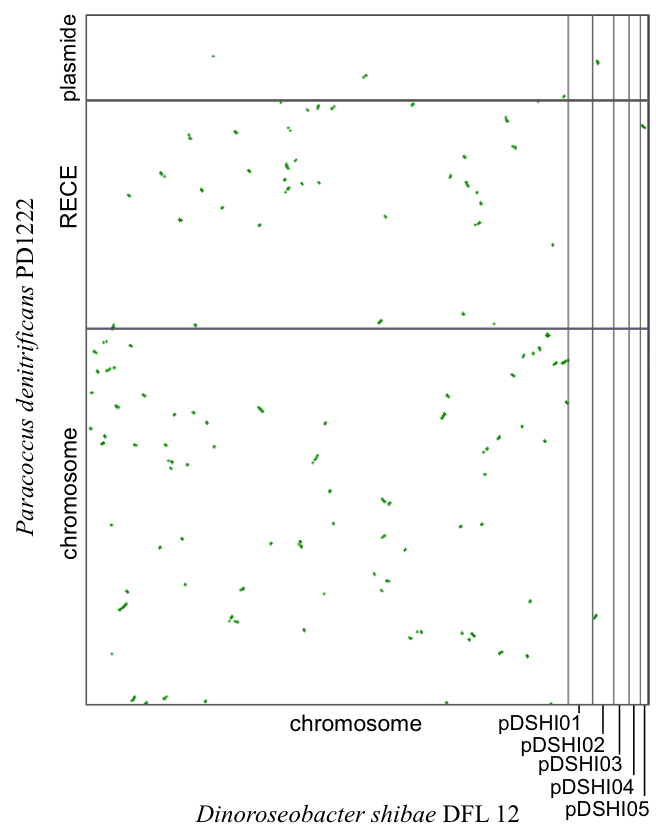
\includegraphics[width=0.5\textwidth]{./img/synteny/new/fig8_1.png}
		\caption[Synténie de \textit{Paracoccus} \textit{vs.} \textit{D. shibae}]{Synténie de \textit{Paracoccus denitrificans} PD1222 (ordonnée) \textit{vs.} \textit{Dinoroseobacter shibae} DFL 12 (abscisse).}\label{figsyntpara1}
		\end{center}
\end{figure}

\begin{table}[H]
\begin{center}
\caption[Valeurs de l'indice synténique pour \textit{Paracoccus}]{Valeurs de l'indice synténique $S_{G}$ (éq. \ref{eqsynteny}) des réplicons de \textit{Paracoccus denitrificans} PD1222 par rapport à ceux des génomes de \textit{Dinoroseobacter shibae} DFL 12 (\ref{tablesyntpara1}) et de \textit{Rhodobacter sphaeroides} ATCC 17029 (\ref{tablesyntpara2}).} 
	\subcaption{\textit{P. denitrificans} PD1222 ($G$) \textit{vs.} \textit{D. shibae} DFL 12 ($G_{ref}$).}\label{tablesyntpara1}
	\begin{tabular}{c|cccccc}
		$G\diagdown G_{ref}$ & $r^{ref}_{chr}$ & $r^{ref}_{pDSHI01}$ & $r^{ref}_{pDSHI02}$ & $r^{ref}_{pDSHI03}$ & $r^{ref}_{pDSHI04}$ & $r^{ref}_{pDSHI05}$\\
		\hline
		$r_{chr}$ & 100 & n.a. & 100 & n.a. & n.a. & n.a.\\
		$r_{RECE}$ & 74 & n.a. & n.a. & 0 & n.a. & n.a.\\
		$r_{plasmide}$ & 12 & n.a. & 677 & n.a. & n.a. & n.a.\\ 
	\end{tabular}
\\ \vspace{1cm}
	\subcaption{\textit{P. denitrificans} PD1222 ($G$) \textit{vs.} \textit{R. sphaeroides} ATCC 17029 ($G_{ref}$).} \label{tablesyntpara2}
	\begin{tabular}{c|ccc}
		$G \diagdown G_{ref}$ & $r^{ref}_{chr}$ & $r^{ref}_{RECE}$ & $r^{ref}_{plasmide}$\\
		\hline
		$r_{chr}$ & 100 & 100 & 100\\
		$r_{RECE}$ & 71 & 59 & 133\\
		$r_{plasmide}$ & 20 & 40 & 0\\ 
	\end{tabular}
\end{center}
\end{table} 
   

\begin{figure}[H]
		\begin{center}
			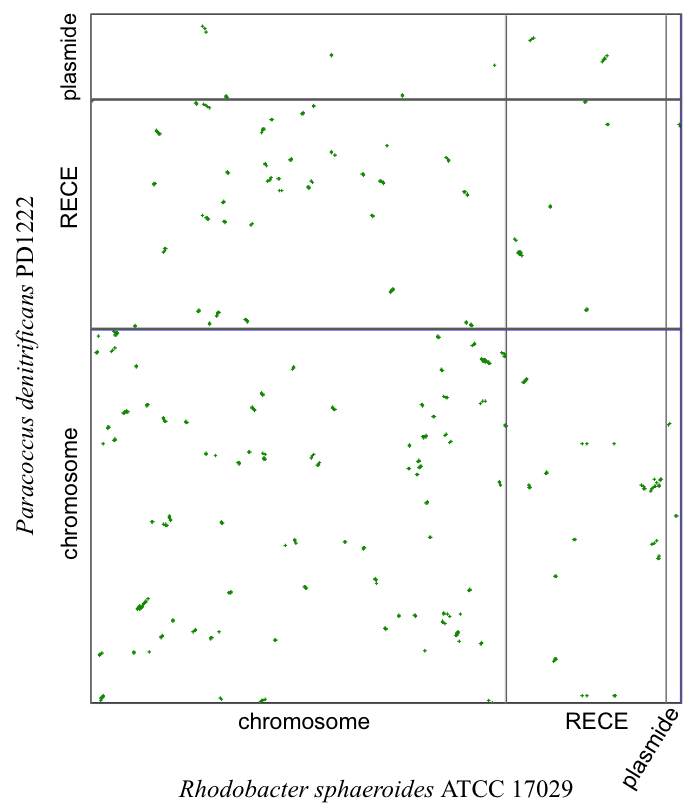
\includegraphics[width=0.5\textwidth]{./img/synteny/new/fig8_2.png}
		\caption[Synténie de \textit{Paracoccus} \textit{vs.}  \textit{R. sphaeroides}]{Synténie de \textit{Paracoccus denitrificans} PD1222 (ordonnée) \textit{vs.}  \textit{Rhodobacter sphaeroides} ATCC 17029 (abscisse).} \label{figsyntpara2}
		\end{center}
\end{figure}

   
Le génome multipartite de \textit{R. sphaeroides} ATCC 17029 est aussi comparé au génome monopartite de \textit{D. shibae} DFL 12 (Figure \ref{figsyntpararhodo}; Table \ref{tablesyntrhodo1})).

\begin{figure}[H]
		\begin{center}
			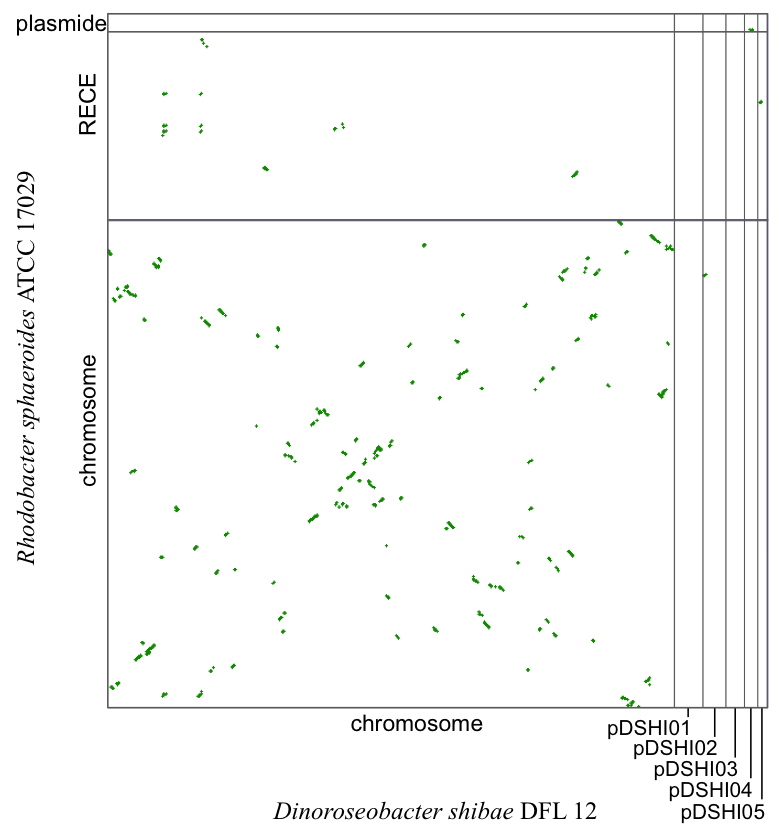
\includegraphics[width=0.5\textwidth]{./img/synteny/new/fig8_3.png}
			\caption[Synténie de \textit{Rhodobacter} \textit{vs.} \textit{D. shibae} ]{Synténie de \textit{R. sphaeroides}  ATCC 17029 (ordonnée) \textit{vs.} \textit{Dinoroseobacter shibae} DFL 12 (abscisse).}\label{figsyntpararhodo}
			\end{center}
\end{figure}


\begin{table}[H]
		\begin{center}
		\caption[Valeurs de l'indice synténique pour \textit{Rhodobacter}]{Valeurs de l'indice synténique $S_{G}$ (éq. \ref{eqsynteny}) entre les réplicons de \textit{Rhodobacter sphaeroides} ATCC 17029 et ceux des génomes  ($G_{ref}$) de \textit{Dinoroseobacter shibae} DFL 12 (\ref{tablesyntrhodo1}) et de \textit{Paracoccus denitrificans} PD1222 (\ref{tablesyntrhodo2}).} \label{tablesyntrhodo}
				\subcaption{\textit{R. sphaeroides}  ATCC 17029 ($G$) \textit{vs.} \textit{D. shibae} DFL 12 ($G_{ref}$).}\label{tablesyntrhodo1}
				\begin{tabular}{c|cccccc}
					$G \diagdown G_{ref}$ & $r^{ref}_{chr}$ & $r^{ref}_{pDSHI01}$ & $r^{ref}_{pDSHI02}$ & $r^{ref}_{pDSHI03}$ & $r^{ref}_{pDSHI04}$ & $r^{ref}_{pDSHI05}$\\
					\hline
					$r_{chr}$ & 100 & n.a. & 100 & n.a. & n.a. & n.a.\\
					$r_{RECE}$ & 17 & n.a. & 0 & n.a. & n.a. & n.a.\\
					$r_{plasmide}$ & 0 & n.a. & 0 & n.a. & n.a. & n.a.\\ 
				\end{tabular}
				\\\vspace{0.5cm}
				\subcaption{\textit{R. sphaeroides} ATCC 17029 ($G$) \textit{vs.} \textit{P. denitrificans} PD1222 ($G_{ref}$).}\label{tablesyntrhodo2}
				\begin{tabular}{c|ccc}
					$G \diagdown G_{ref}$ & $r^{ref}_{chr}$ & $r^{ref}_{RECE}$ & $r^{ref}_{plasmide}$\\
					\hline
					$r_{chr}$ & 100 & 100 & 100\\
					$r_{RECE}$ & 50 & 42 & 110\\
					$r_{plasmide}$ & 26 & 49 & 0\\ 
				\end{tabular}
		\end{center}
\end{table} 
    
	Il existe une synténie plus importante entre le RECE de \textit{P. denitrificans} PD1222 et les chromosomes de \textit{D. shibae} DFL 12 (Table \ref{tablesyntpara1}) et de \textit{R. sphaeroides} ATCC 17029 (Table \ref{tablesyntpara2}) qu'entre le RECE de \textit{R. sphaeroides} ATCC 17029 et les chromosomes de \textit{P. denitrificans} PD1222 (Table \ref{tablesyntrhodo2}) et de \textit{D. shibae} DFL 12 (Table \ref{tablesyntrhodo1}). Une faible synténie est de plus présente entre les RECE des deux espèces à génome multipartite \textit{P. denitrificans} PD1222 et \textit{R. sphaeroides} ATCC 17029 (Tables \ref{tablesyntpara2} et \ref{tablesyntrhodo2}). On peut donc supposer que \textbf{les deux RECE sont issus d'événements évolutifs distincts ou évoluent plus vite} (Figure \ref{figsyntpara2}). En comparant le génome de \textit{P. denitrificans} PD1222 avec des génomes phylogéniquement plus distants: \textit{Maricaulis mari} MCS10 (Rhodobactérales) et \textit{Caulobacter crescentus}  CB15 (Caulobactérales), des valeurs similaires sont observées malgré des signaux synténiques beaucoup plus faibles (résultats non montrés).\\
	Il a été suggéré que certains plasmides des Rhodobactérales, dont deux de \textit{D. shibae} DFL 12, sont en fait des ``chromids" en raison de leur origine de réplication atypique \citep{Petersen2013}. Nos précédentes analyses n'ont pas identifié de spécificités caractéristiques des RECE parmi la majorité des réplicons des genres des \textit{Roseobacter/Dinoroseobacter} et ces analyses synténiques n'indiquent pas davantage de possibles transferts entre ces réplicons et les chromosomes (Tables \ref{tablesyntpara1} et \ref{tablesyntrhodo1}).
\\ \\
	 Les bactéries du genre \textit{Ruegeria}, appartenant également à la famille des Rhodobacteraceae, sont des espèces marines. Les espèces \textit{R. pomeyori} et \textit{R.} sp. TM1040 possèdent chacune un mégaplasmide. Parmi les plasmides des \textit{Rhodobacteraceae}, seul le mégaplasmide de \textit{R.} sp. TM1040, avec celui de \textit{Paracoccus}, présente des spécificités de RECE (\textit{cf.} Chapitre \ref{classifsupervisee}). Le génome de \textit{Ruegeria} sp. TM1040 a donc été comparé à celui de \textit{D. shibae DFL 12} (Figure \ref{figsyntruegdino}; Table \ref{tablesyntrug}). \textit{blastn} est utilisé.

\begin{figure}[H]
   \begin{center}
   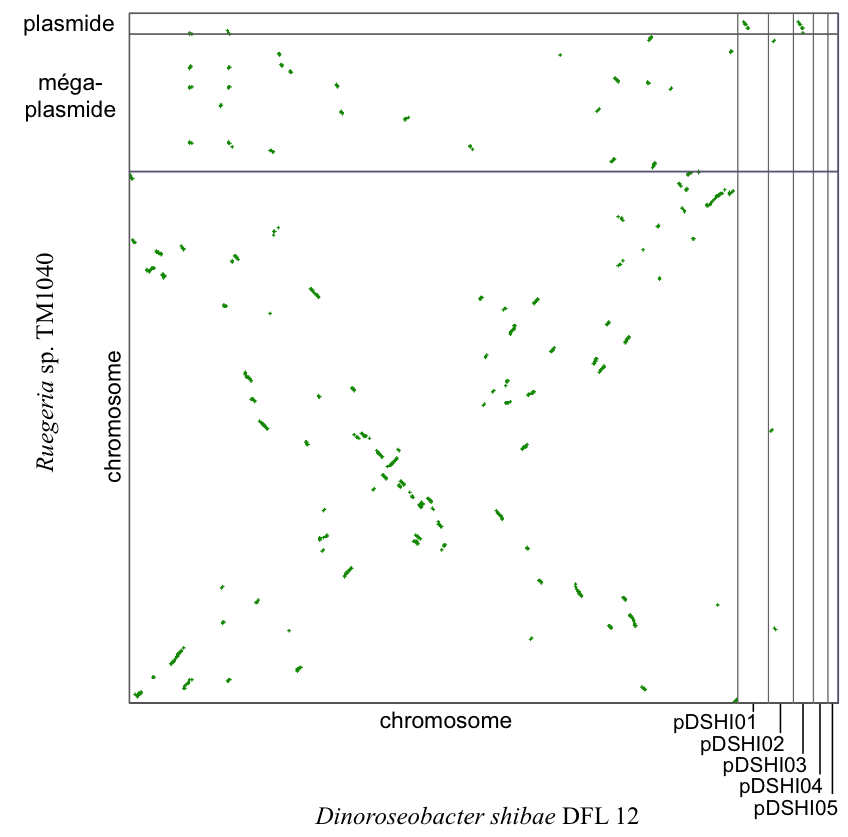
\includegraphics[width=0.5\textwidth]{./img/synteny/new/fig8_4.png}
   \caption[Synténie de \textit{Ruegeria} \textit{vs.} \textit{D. shibae} ]{Synténie de \textit{Ruegeria} sp. TM1040 (ordonnée) \textit{vs.} \textit{Dinoroseobacter shibae}  DFL 12 (abscisse).}\label{figsyntruegdino}
   \end{center}
\end{figure}     
  
\begin{table}[H]
	\begin{center}
	\caption[Valeurs de l'indice synténique pour \textit{Ruegeria}]{Valeur de l'indice synténique $S_{G}$ (éq. \ref{eqsynteny}) entre les réplicons de \textit{Ruegeria} sp. TM1040 ($G$) et ceux du génome de \textit{Dinoroseobacter shibae} DFL 12 ($G_{ref}$).}\label{tablesyntrug}
		\begin{tabular}{c|cccccc}
		$G \diagdown G_{ref}$ & $r^{ref}_{chr}$ & $r^{ref}_{pDSHI01}$ & $r^{ref}_{pDSHI02}$ & $r^{ref}_{pDSHI03}$ & $r^{ref}_{pDSHI04}$ & $r^{ref}_{pDSHI05}$\\
		\hline
		$r_{chr}$ & 100 & n.a. & 100 & n.a. & n.a. & n.a.\\
   		$ r_{megaplasmide}$ & 62 & n.a. & 0 & n.a. & n.a. & n.a.\\
  		$r_{plasmide}$ & 23 & n.a. & 126 & n.a. & n.a. & n.a.\\ 
		\end{tabular}
	\end{center}
\end{table}
   
   Le mégaplasmide de \textit{Ruegeria} sp. TM1040 possède de larges zones synténiques avec le chromosome de \textit{D. shibae DFL 12}. La synténie est largement plus importante que dans le cas du RECE de \textit{R. sphaeroides} avec le même chromosome de \textit{D. shibae} relativement à la synténie partagée avec les chromosomes de \textit{Ruegeria} sp. TM1040 et de \textit{R. sphaeroides} (résultats non montrés). Cette caractéristique est de plus retrouvée en comparant le génome de \textit{Ruegeria} sp. TM1040 à celui de \textit{P. denitrificans} PD1222 (résultats non montrés). Le mégaplasmide de \textit{Ruegeria} sp. TM1040 a donc une très forte probabilité d'être un RECE. Par contre, aucune région de synténie n'est detectée avec le RECE de \textit{P. denitrificans} PD1222, ce qui suggère que le mégaplasmide/RECE de \textit{Ruegeria} sp. TM1040 et le RECE de \textit{P. denitrificans} PD1222 ont des origines différentes.


\subsection{Analyse des Caulobactérales et des Sphingomonadales}
\subsubsection{Caulobactérales}\label{parasti}
   Le génome d'\textit{Asticcacaulis excentricus} CB 48 a été comparé à ceux de \textit{Caulobacter crescentus} CB15, d'\textit{Erythrobacter litoralis} HTCC2594 et de \textit{Zymomonas mobilis} subsp. \textit{mobilis} NCIMB 11163 (Figure \ref{figsyntasticca}). Les genres \textit{Asticaccaulis} et \textit{Caulobacter} appartiennent à la famille des Caulobacteraceae alors que \textit{Erythrobacter} et \textit{Zymomonas} sont des Sphingomonadaceae.  \textit{blastn} est utilisé. 

\begin{figure}[H]
	\begin{center}
	\begin{minipage}{0.5\textwidth}
	\centering
	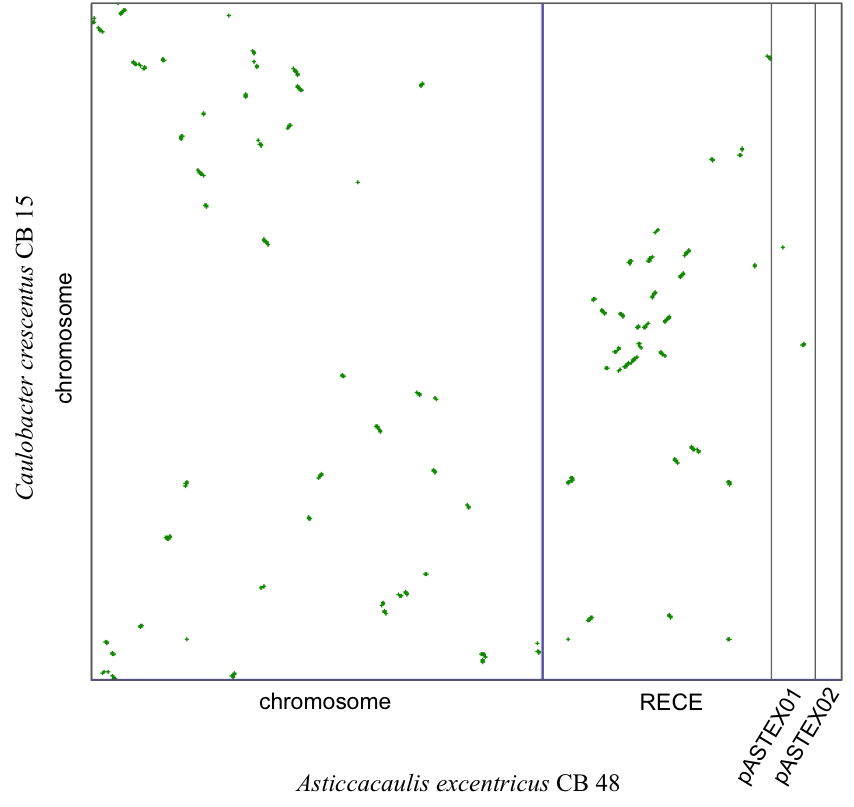
\includegraphics[width=0.8\textwidth]{./img/synteny/new/fig8_5a.png}
   	\subcaption{\textit{A. excentricus} CB 48 (ordonnée) \textit{vs.}  \textit{Caulobacter crescentus} CB15 (abscisse).}\label{figsyntasticca1}
	\end{minipage}
	\end{center} 

	\begin{center}
	\begin{minipage}{0.5\textwidth}
	\centering
	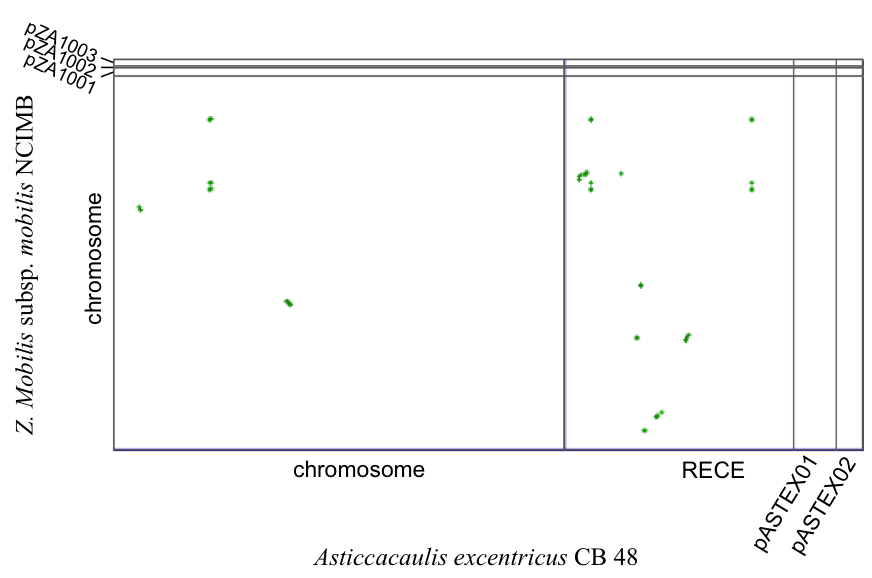
\includegraphics[width=0.8\textwidth]{./img/synteny/new/fig8_5b.png}
	\subcaption{\textit{A. excentricus} CB 48 (ordonnée) \textit{vs.}  \textit{Zymomonas mobilis} subsp. \textit{mobilis} NCIMB 11163 (abscisse).}\label{figsyntasticca2}
	\end{minipage}
	\end{center} 

	\begin{center}
	\begin{minipage}{0.5\textwidth}
	\centering
	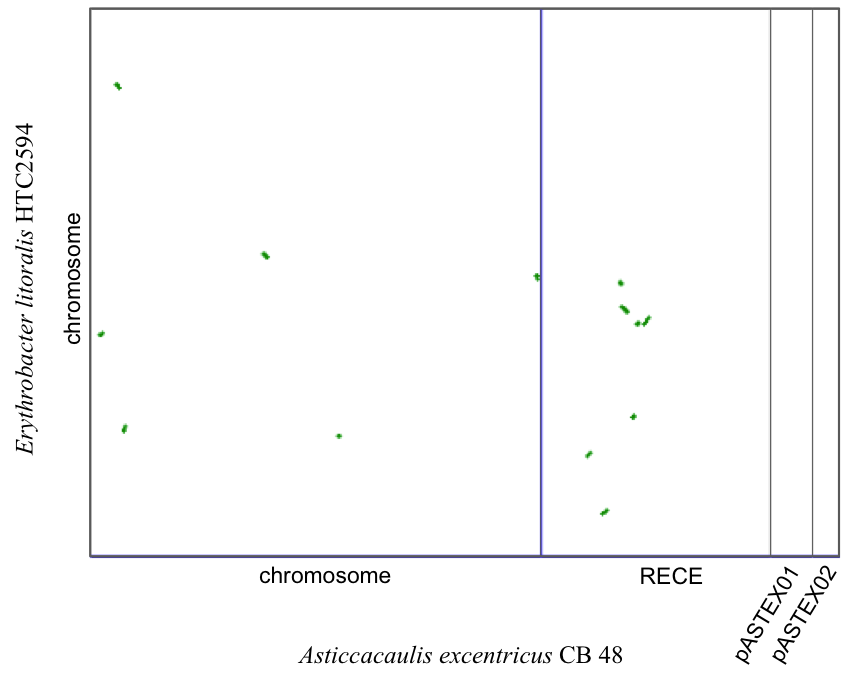
\includegraphics[width=0.8\textwidth]{./img/synteny/new/fig8_5c.png}
	\subcaption{\textit{A. excentricus} CB 48 (ordonnée) \textit{vs.}  \textit{Erythrobacter litoralis} HTCC2594 (abscisse).}\label{figsyntasticca3}
	\end{minipage}
	\end{center} 
\caption[Synténie d'\textit{Asticcacaulis} \textit{vs.} autre Caulobacteraceae et Sphingomonaceae]{Synténie entre \textit{Asticcacaulis excentricus} CB 48 (abscisse) et \textit{Caulobacter crescentus} CB15 (ordonnée; \ref{figsyntasticca1}), \textit{Zymomonas mobilis} subsp. \textit{mobilis} NCIMB 11163 (ordonnée; \ref{figsyntasticca2}), et \textit{Erythrobacter litoralis }HTCC2594 (ordonnée; \ref{figsyntasticca2}).} \label{figsyntasticca}
\end{figure}

\begin{table}[H]
	\begin{center}   
	\caption[Valeurs de l'indice synténique pour \textit{Asticcacaulis}]{Valeurs de l'indice synténique $S_{G}$ (éq. \ref{eqsynteny}) entre les réplicons du génome d'\textit{Asticcacaulis excentricus} CB 48 et ceux des génomes de \textit{Caulobacter crescentus} CB15 (\ref{tablesyntsphing1}), \textit{Erythrobacter litoralis} HTCC2594 (\ref{tablesyntsphing2}), et \textit{Zymomonas mobilis} subsp. \textit{mobilis} NCIMB 11163 (\ref{tablesyntsphing3}).}\label{tablesyntasticca}
	\begin{minipage}[t]{0.45\textwidth}
	\centering
	\subcaption{\textit{A. excentricus} CB 48 ($G$) \textit{vs.} \textit{C. crescentus} CB15 ($G_{ref}$).}\label{tablesyntAstic1}
		\begin{tabular}{c|c}
		$G \diagdown G_{ref}$ & $r^{ref}_{chr}$\\
		\hline
		$r_{chr}$ & 100\\
		$ r_{RECE}$ & 170\\
		$r_{pASTEX01}$ & 40\\ 
		$r_{pASTEX02}$ & 0\\
		\end{tabular} 
	\end{minipage}
	\hspace{1cm}
	\begin{minipage}[t]{0.45\textwidth}
	\centering
	\subcaption{\textit{A. excentricus} CB 48 ($G$) \textit{vs.} \textit{E. litoralis }HTCC2594 ($G_{ref}$).}\label{tablesyntAstic2}
  		\begin{tabular}{c|cccc}
		$G \diagdown G_{ref}$ & $r^{ref}_{chr}$\\
		\hline
		$r_{chr}$ & 100\\
		$ r_{RECE}$ & 194\\
		$r_{pASTEX01}$ & 0\\ 
		$r_{pASTEX02}$ & 0\\
		\end{tabular}
	\end{minipage}
	\end{center} 

\begin{center}   
	\begin{minipage}[t]{0.45\textwidth}
	\centering
	\subcaption{\textit{A. excentricus} CB 48 ($G$) \textit{vs.}\textit{Z. mobilis} NCIMB 11163 ($G_{ref}$).}\label{tablesyntAstic3}
	\hspace*{-1.5cm}
		\begin{tabular}{c|cccc}
		$G \diagdown G_{ref}$ & $r^{ref}_{Mpl}$ & $r^{ref}_{pZA1001}$ & $r^{ref}_{pZA1002}$ & $r^{ref}_{pZA1003}$\\
		\hline
		$r_{chr}$ & 100 & n.a. & n.a. & n.a. \\
		$ r_{RECE}$ & 470 & n.a. & n.a. & n.a. \\
		$r_{pASTEX01}$ & 0 & n.a. & n.a. & n.a. \\ 
		$r_{pASTEX02}$ & 0 & n.a. & n.a. &  n.a. \\
		\end{tabular}
	\end{minipage} 
\end{center} 
\end{table}   

   De façon surprenante, les valeurs de l'indice $S_{G}$ sont presque deux fois supérieures pour le RECE que pour le chromosome d'\textit{Asticcacaulis excentricus} CB 48 (\ref{figsyntasticca}) indiquant que la co-linéarité est quasiment deux fois plus conservée sur le RECE. \textbf{\color{orange}La zone de synténie du RECE d'\textit{A. excentricus} CB 48 avec le chromosome de \textit{C. crescentus} CB15 semble se superposer à une zone sur le chromosome d'\textit{A. excentricus} CB 48 où il y a une absence de synténie avec le chromosome de \textit{C. crescentus} CB15} (Figure \ref{figsyntasticca1}). Plus étonnant, on observe, comparativement au chromosome d'\textit{Asticcacaulis}, un niveau de synténie similaire du RECE avec le chromosome d'\textit{Erythrobacter litoralis} HTCC2594 (Table \ref{tablesyntsphing2}) et une synténie 5 fois supérieure avec le chromosome de \textit{Zymomonas mobilis} subsp. \textit{mobilis} NCIMB 11163 (Table \ref{tablesyntAstic3}). Cependant, compte-tenu des signaux synténiques très atténués pour les comparaisons des chromosomes avec \textit{Zymomonas} et \textit{Erythrobacter}, ces derniers résultats sont à interpréter avec prudence (\textit{cf.} comparaison \textit{Caulobacter/Sphingobium} ci-dessous). 
 
 
\subsubsection{Sphingomonadales}\label{parsphi}
	 Le génome de \textit{Sphingobium japonicum} NBRC 101211 est comparé à ceux de \textit{Caulobacter crescentus} NA1000, \textit{Novosphingobium} sp. PP1Y et \textit{Zymomonas mobilis} subsp. \textit{pomaceae} ATCC 29192. \textit{Sphingobium}, \textit{Novosphingobium} et \textit{Zymomonas} appartiennent aux Sphingomonadaceae, \textit{Novosphingobium} étant plus proche phylogéniquement de \textit{Sphingobium} que \textit{Zymomonas}. \textit{Caulobacter} appartenant aux Caulobacteraceae est le plus distant de \textit{Sphingobium}.

\begin{figure}[H]
\begin{center}
	\begin{minipage}{0.49\textwidth}
	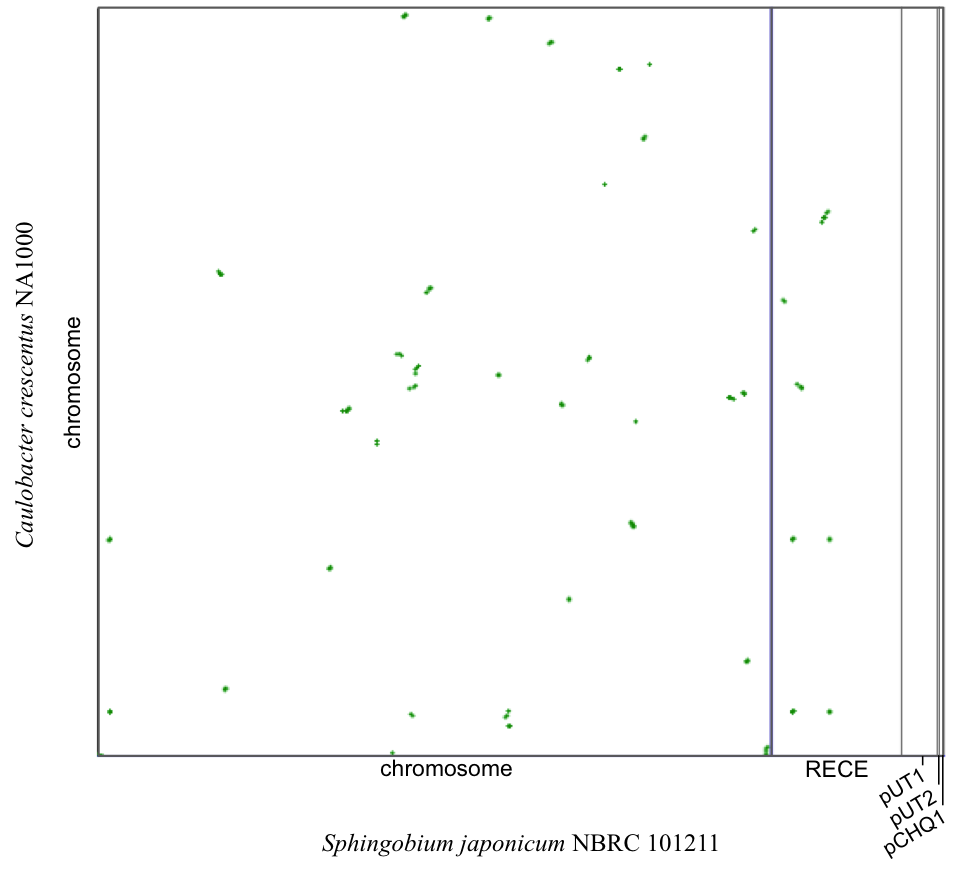
\includegraphics[width=\textwidth]{./img/synteny/new/fig8_6a.png}
	\subcaption{\textit{Sphingobium japonicum} NBRC 101211 (ordonnée) \textit{vs.} \textit{Caulobacter crescentus} NA1000 (abscisse).}\label{figsyntsphing1}
	\end{minipage}
	\begin{minipage}{0.49\textwidth}
	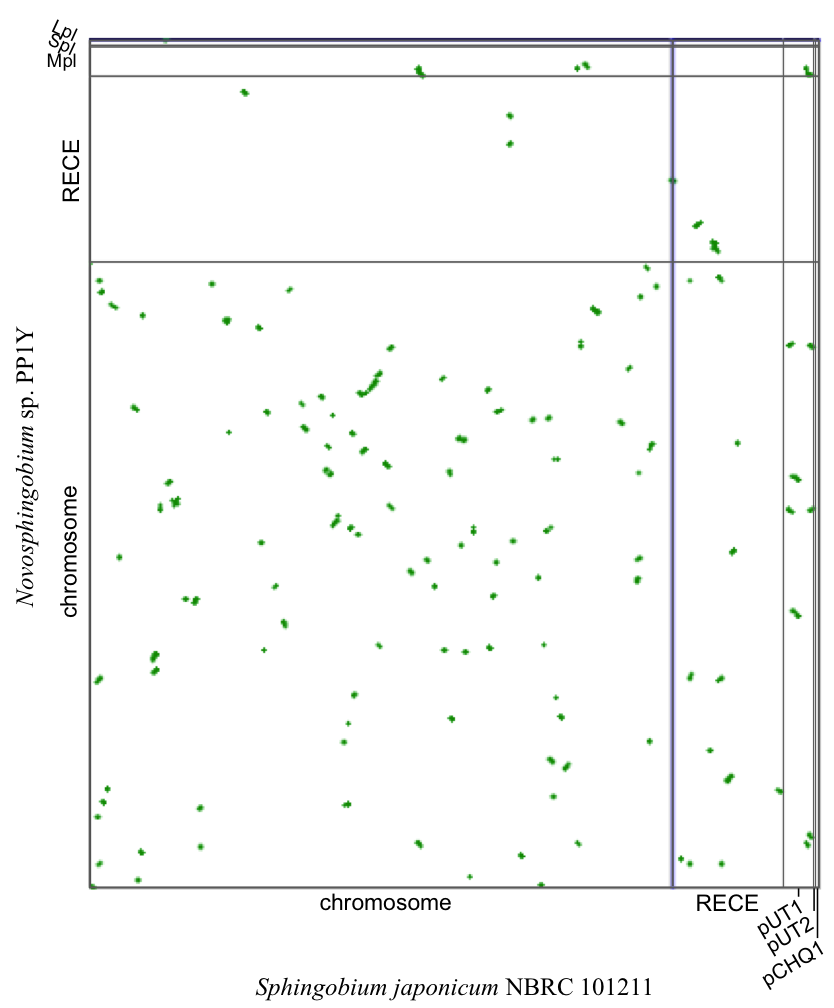
\includegraphics[width=1.1\textwidth]{./img/synteny/new/fig8_6b.png}
	\subcaption{\textit{Sphingobium japonicum} NBRC 101211 (ordonnée) \textit{vs.} \textit{Novosphingobium} sp. PP1Y (abscisse).}\label{figsyntsphing2}
	\end{minipage}

	\begin{minipage}{0.7\textwidth}
	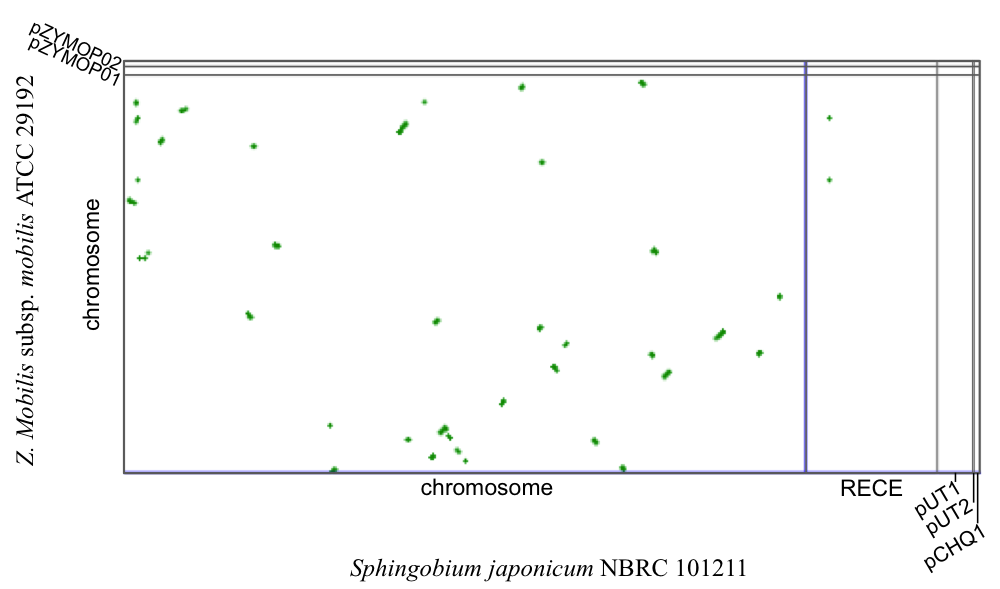
\includegraphics[width=\textwidth]{./img/synteny/new/fig8_6c.png}
	\subcaption{\textit{Sphingobium japonicum} NBRC 101211 (ordonnée) \textit{vs.} \textit{Zymomonas mobilis} subsp. \textit{pomaceae} ATCC 29192 (abscisse).}\label{figsyntsphing3}
	\end{minipage}

\caption[Synténie de \textit{Sphingobium} \textit{vs.}  Caulobacteraceae et autres Sphingomonadaceae]{Synténie entre \textit{Sphingobium japonicum} NBRC 101211 (ordonnée) et \textit{Caulobacter crescentus} NA1000 (abcisse; \ref{figsyntsphing1}), \textit{Novosphingobium} sp. PP1Y (abcisse; \ref{figsyntsphing2}) et \textit{Zymomonas mobilis} subsp. \textit{pomaceae} ATCC 29192 (abcisse; \ref{figsyntsphing3}).}\label{figsyntsphing}
\end{center}
\end{figure} 

\begin{table}[H]
\begin{center}
\caption[Valeurs de l'indice synténique pour \textit{Sphingobium}]{Valeurs de l'indice synténique $S_{G}$ (éq. \ref{eqsynteny}) entre les réplicons du génome de \textit{Sphingobium japonicum} NBRC 101211 et ceux des génomes de \textit{Caulobacter crescentus} NA1000 (\ref{tablesyntsphing1}), \textit{Novosphingobium} sp. PP1Y (\ref{tablesyntsphing2}), et \textit{Zymomonas mobilis} subsp. \textit{pomaceae} ATCC 29192 (\ref{tablesyntsphing3}).}\label{tablesyntsphing}
	\begin{minipage}[t]{0.45\textwidth}
	\subcaption{\textit{S. japonicum} NBRC 101211 ($G$) \textit{vs.} \textit{Caulobacter crescentus} NA1000 ($G_{ref}$).}\label{tablesyntsphing1}
		\begin{tabular}{c|c}
		$G \diagdown G_{ref}$ & $r^{ref}_{chr} $\\
		\hline
		$r_{chr}$ & 100\\
		$ r_{RECE}$ & 96\\
		$r_{pUT1}$ & 0\\ 
		$r_{pUT2}$ & 0\\ 
		$r_{pCHQ1}$ & 0\\ 
		\end{tabular}
	\end{minipage}
\hspace{1cm}
	\begin{minipage}[t]{0.45\textwidth}
	\subcaption{\textit{S. japonicum} NBRC 101211 ($G$) \textit{vs.} \textit{Novosphingobium} sp. PP1Y ($G_{ref}$).}\label{tablesyntsphing2}
		\begin{tabular}{c|cccc}
		$G \diagdown G_{ref}$ & $r^{ref}_{chr}$ & $r^{ref}_{Mpl}$ & $r^{ref}_{Lpl}$ & $r^{ref}_{Spl}$\\
		\hline
		$r_{chr}$ & 100 & 100 & 100 & 100\\
		$ r_{RECE}$ & 70 & 0 & 980 & 0\\
		$r_{pUT1}$ & 0 & 0 & 0 & 0\\ 
		$r_{pUT2}$ & 0 & 0 & 0 & 0\\ 
		$r_{pCHQ1}$ & 249 & 1041 & 0 & 0\\ 
		\end{tabular}
	\end{minipage}
\end{center}
\vspace*{0.5cm}
\centering
\hspace*{-1cm}
	\begin{minipage}[t]{0.45\textwidth}
		\begin{tabular}{c|ccc}
		$G \diagdown G_{ref}$ & $r^{ref}_{Mpl}$ & $r^{ref}_{pZYMOP01}$ & $r^{ref}_{pZYMOP02}$ \\
		\hline
		$r_{chr}$ & 100 & n.a. & n.a.\\
		$ r_{RECE}$ & 17 & n.a. & n.a. \\
		$r_{pUT1}$ & 0 & n.a. & n.a.\\ 
		$r_{pUT2}$ & 0 & n.a. & n.a.\\ 
		$r_{pCHQ1}$ & 0 & n.a. & n.a.\\ 
		\end{tabular}
	 \subcaption{\textit{S. japonicum} NBRC 101211 ($G$) \textit{vs.} \textit{Z. mobilis } ATCC 29192 ($G_{ref}$).}\label{tablesyntsphing3}
	\end{minipage}
\end{table}

   La synténie du RECE de \textit{Sphingobium}, relativement importante avec le chromosome de \textit{Novosphingobium}, devient faible avec le chromosome \textit{Zymomonas} et disparaît complètement avec celui d'\textit{Erythrobacter litoralis} HTCC2594, une autre Sphingomonadaceae (résultats non montrés). Elle reste cependant relativement importante avec le chromosome de \textit{Caulobacter}, représentant d'une autre famille (Caulobacteraceae). Il apparaît clair qu'il existe une zone nucléotidique commune entre le RECE et le plasmide de \textit{Novosphingobium} (Figure \ref{figsyntsphing2}), témoignant de l'origine plasmidique du RECE. De nombreuses zones synténiques sont de plus trouvées entre le chromosome de \textit{Novosphingobium} et le plasmide pCHQ1 de \textit{Sphingobium}, suggérant l'intégration d'un certain nombre de gènes plasmidiques dans le chromosome de \textit{Novosphingobium}. Le plasmide pCHQ1 est de plus identifié, avec un faible indice de confiance, comme potentiel RECE (\textit{cf.} Chapitre \ref{classifsupervisee}) indiquant une éventuelle transition plasmide/RECE pour ce réplicon.\\
    Il est assez intriguant de retrouver un indice synténique relativement fort entre le chromosome de \textit{Caulobacter} et le RECE de \textit{Sphingobium}. Cette synténie est due, entre autres, à l'identification de gènes d'ARN ribosomiques. Compte-tenu de la faible synténie entre les chromosomes de \textit{Sphingobium} et \textit{Caulobacter}, on peut considérer que cette valeur de l'indice synténique n'est pas forcément représentative d'une conservation de région synténique chez le RECE car aucune synténie n'est retrouvée avec les réplicons, RECE et chromosome, de \textit{Zymomonas} et le chromosome de \textit{Erythrobacter}, mais reflète plutôt la faible synténie entre les deux chromosomes. 
        

\subsection{Analyse des Rhizobiales}\label{parbruc} 
   Le génome de \textit{Brucella melitensis} biovar Abortus 2308 est comparé aux génomes de \textit{Bartonella australis} Aust/NH1, \textit{Mesorhizobium loti} MAFF303099, \textit{Sinorhizobium meliloti} 1021, \textit{Rhizobium etli}CFN 42, \textit{Agrobacterium vitis} S4, \textit{Agrobacterium tumefaciens} C58 et \textit{Bradyrhizobium japonicum} USDA 110, bactéries qui font toutes partie des Rhizobiales (Figure \ref{figphylrhizo}). Last est utilisé en raison de la grande taille de certains génomes (Figure \ref{figsyntbruc} et Table \ref{tablesyntbruc}).
      
	La plupart de ces espèces sont connues pour leur capacité à fixer le di-azote atmosphérique et à s'associer symbiotiquement avec les plantes de la famille des Légumineuses au niveau de leurs racines et parfois de leur tiges. Ces espèces sont de plus les hôtes de RECE, plasmides et mégaplasmides caractéristiques \citep{Pinto2012}, ayant une origine de réplication spécifique, comprenant un opéron \textit{repABC}. L'histoire évolutive de leur génome apparaît étroitement liée à celle de leurs mégaplasmides. En particulier, il a été suggéré que les RECE des Rhizobiales dérivent d'un mégaplasmide \textit{repABC} ancestral (``plasmide ITR" pour \textit{\textbf{I}ntragenomic \textbf{T}ranslocation \textbf{R}ecipient}) ayant capturé certains gènes du chromosome \citep{Slater2009} (Figure \ref{figphylrhizo}).     

\begin{figure}[h]
	\begin{center}
		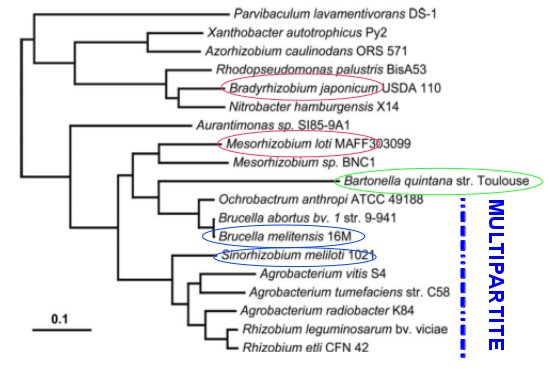
\includegraphics[width=0.8\textwidth]{./img/figphylrhizo_3.png}
	\end{center}
	\caption[Hypothèse d'évolution du plasmide ITR chez les Rhizobiales]{Hypothèse d'évolution du plasmide ITR chez les Rhizobiales.\\ Plasmide ITR : transformé en RECE (bleu), intégré dans le chromosome (rouge), ou perdu (vert). Adaptée de \citep{Slater2009}.} \label{figphylrhizo}
\end{figure}

Les plasmides/mégaplasmides \textit{repABC} ne suivent cependant pas une évolution verticale et sont soumis à de nombreux réarrangements et échanges inter- et intragénomiques \citep{Slater2009,Castillo-Ramirez2009}. De plus, de nombreuses études ont montré la plus grande variabilité des RECE des Rhizobiales par rapport aux chromosomes \citep{Slater2009,Bavishi2010}. \textit{Brucella melitensis} est un endosymbiote facultatif ayant un génome relativement petit (3.1 Mb), cette taille réduite pouvant être le résultat de leur état endosymbiotique \citep{Wattam2009}. Les transferts des gènes chromosomiques sur le plasmide ITR semblent avoir eu lieu indépendamment chez les Brucellaceae: 25 clusters de gènes transférés du chromosome au RECE identifiés en comparaison, chez les Rhizobiaceae, d'un seul cluster commun identifié sur pSymB de \textit{S. meliloti} et d'au moins deux clusters communs chez \textit{Rhizobium} \citep{Slater2009}. \textit{Rhizobium} et \textit{Agrobacterium} ont des plasmides ITR relativement proches, mais le RECE d'\textit{A. tumefaciens} est linéaire contrairement à celui d'\textit{A. vitis} \citep{lassalle2013genomes}. Enfin, chez \textit{Bradyrhizobium} et \textit{Mesorhizobium}, le plasmide ITR serait intégré dans le chromosome, alors que pour d'autres espèces (dont \textit{Bartonella}) le plasmide ITR aurait été perdu \citep{Slater2009}. \textbf{Les Rhizobiales représentent donc un jeu de données essentiel dans la comparaison des taux de synténie entre génomes multi- et monopartites.}

   
\begin{figure}[H]
\begin{center}
\hspace*{-3cm}
	\begin{minipage}{0.5\textwidth}
		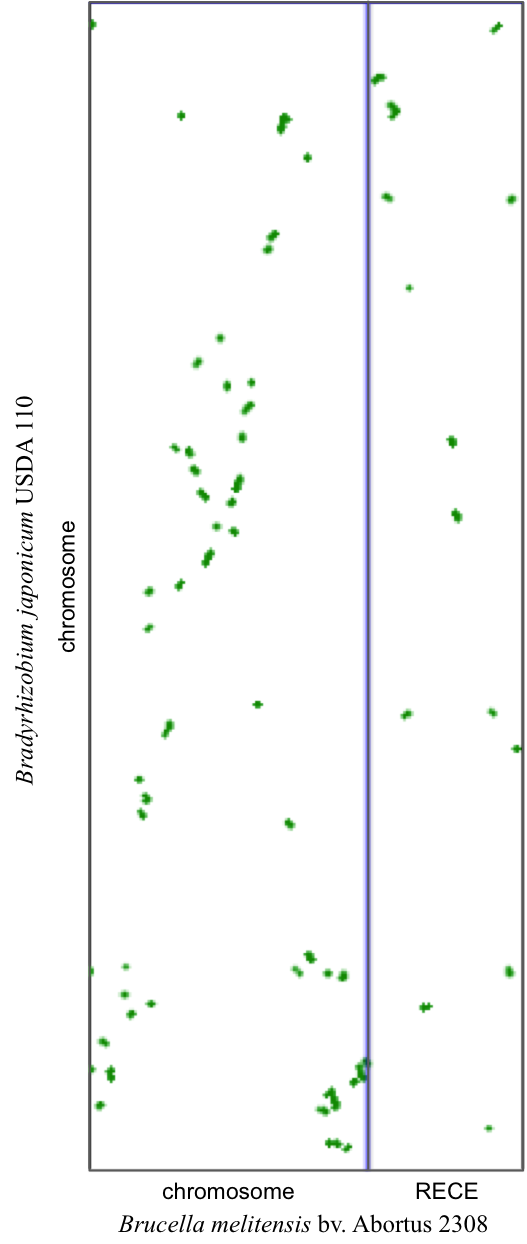
\includegraphics[width=\textwidth]{./img/synteny/new/fig8_8d.png}
		\subcaption{\mbox{\textit{B. melitensis}} 2308 (ordonnée) \textit{vs.} \textit{B. japonicum} USDA 110 (abscisse).}\label{figsyntbruc4}
	\end{minipage}
	\begin{minipage}{0.5\textwidth}
		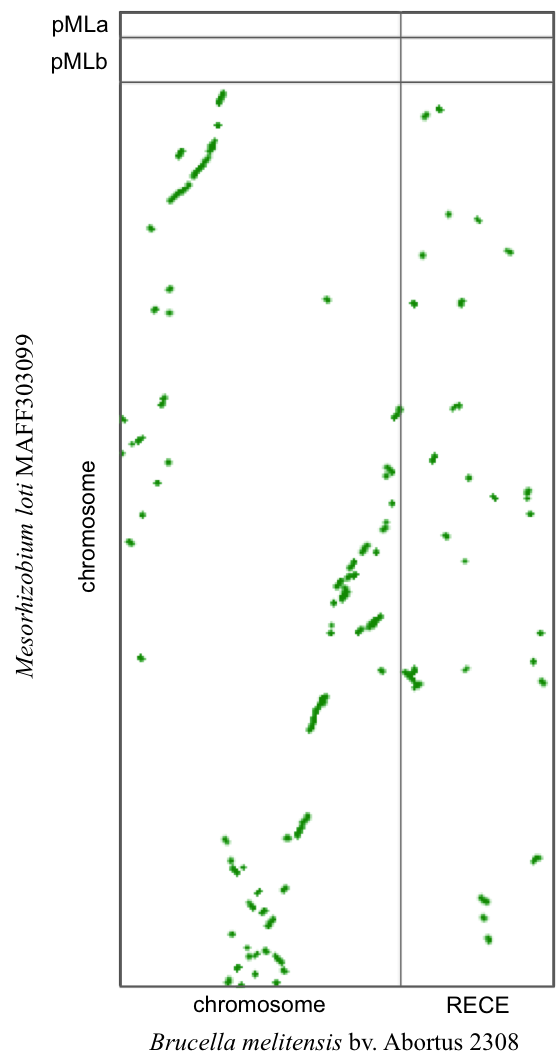
\includegraphics[width=1.1\textwidth]{./img/synteny/new/fig8_8b.png}
		\subcaption{\textit{B. melitensis} 2308 (ordonnée) \textit{vs.} \textit{M. loti} MAFF303099 (abscisse).}\label{figsyntbruc2}
	\end{minipage}
	\end{center}
\end{figure}

\begin{figure}[H]
\begin{center}
\hspace*{-3cm}
	\begin{minipage}{0.5\textwidth}
		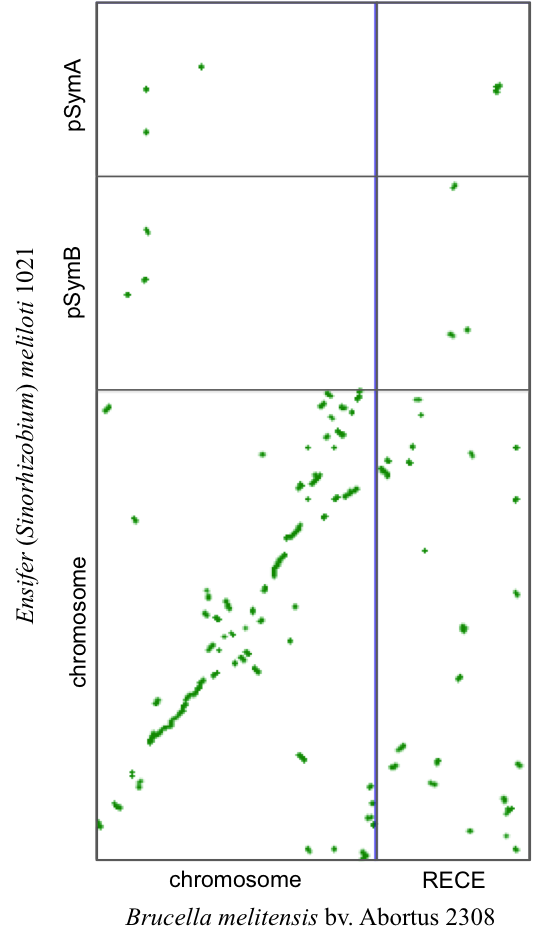
\includegraphics[width=\textwidth]{./img/synteny/new/fig8_8c.png}
		\subcaption{\textit{B. melitensis} 2308 (ordonnée) \textit{vs.} \textit{S. meliloti} 1021 (abscisse).}\label{figsyntbruc3}
	\end{minipage}
	\begin{minipage}{0.5\textwidth}
		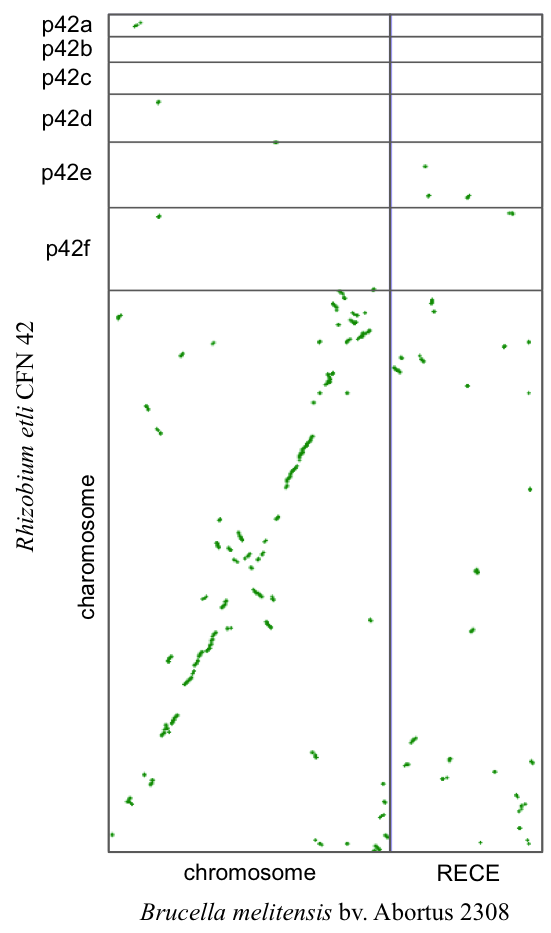
\includegraphics[width=\textwidth]{./img/synteny/new/fig8_8e.png}
		\subcaption{\textit{B. melitensis} 2308 (ordonnée) \textit{vs.} \textit{R. etli} CFN 42 (abscisse).}\label{figsyntbruc5}
	\end{minipage}
\\
\centering
	\begin{minipage}{0.5\textwidth}
		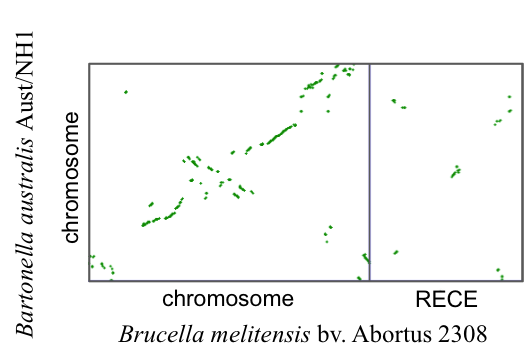
\includegraphics[width=\textwidth]{./img/synteny/new/fig8_8a.png}
		\subcaption{\textit{B. melitensis} 2308 (ordonnée) \textit{vs.} \textit{B. australis} Aust/NH1 (abscisse).}\label{figsyntbruc1}
	\end{minipage}
\end{center}
\end{figure}

\begin{figure}[H]
\begin{center}
	\begin{minipage}{0.5\textwidth}
		%\centering
		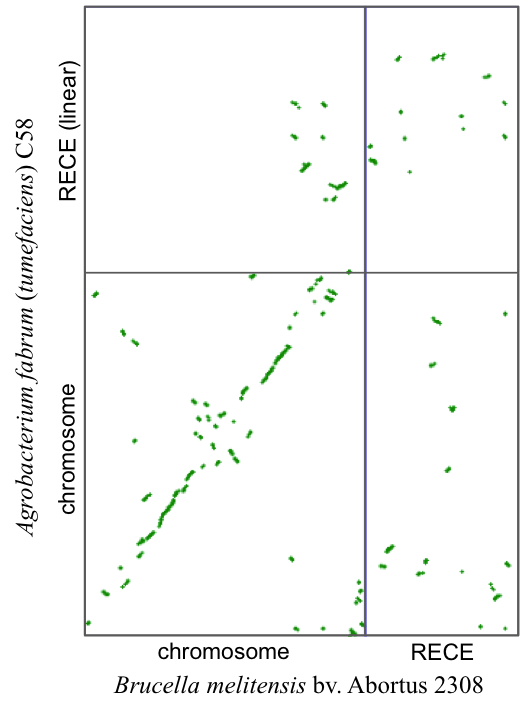
\includegraphics[width=\textwidth]{./img/synteny/new/fig8_8g.png}
		\subcaption{\textit{B. melitensis} 2308 (ordonnée) \textit{vs.} \textit{A. tumefaciens} (abscisse).}\label{figsyntbruc7}
	\end{minipage}
	\begin{minipage}{0.5\textwidth}
		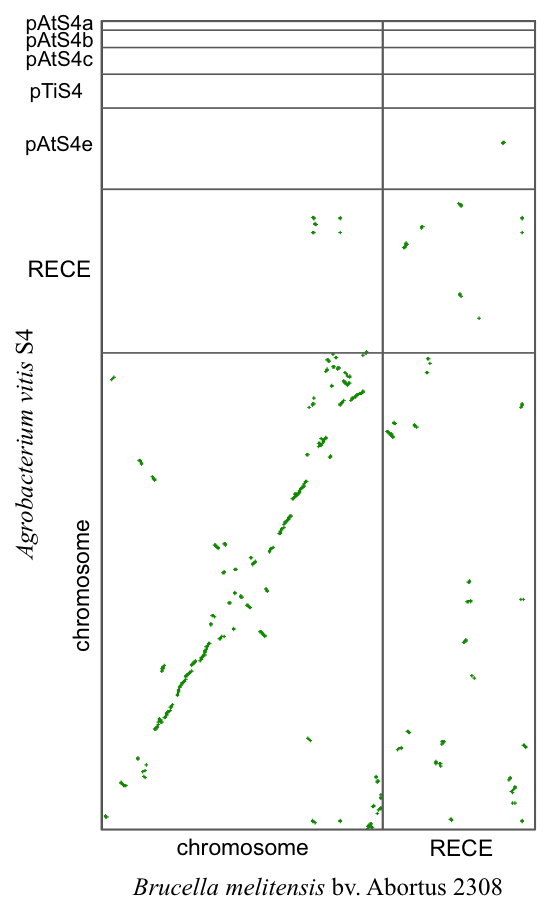
\includegraphics[width=\textwidth]{./img/synteny/new/fig8_8f.png}
		\subcaption{\textit{B. melitensis} 2308 (ordonnée) \textit{vs.} \textit{A. vitis} S4 (abscisse).}\label{figsyntbruc6}
	\end{minipage}
\end{center}
\hspace{-3cm}
\end{figure}  

\captionof{figure}[Synténie de \textit{Brucella} \textit{vs.} autres Rhizobiales]{Synténie de \textit{Brucella melitensis} bv. Abortus 2308 avec les génomes monopartites de \textit{Bartonella australis} Aust/NH1 (\ref{figsyntbruc1}), \textit{Bradyrhizobium japonicum} USDA 110 (\ref{figsyntbruc4}), \textit{Mesorhizobium loti} MAFF303099 (\ref{figsyntbruc2}), \textit{Sinorhizobium meliloti} 1021 (\ref{figsyntbruc3}) et \textit{Rhizobium etli} CFN 42 (\ref{figsyntbruc5}), et les génomes multipartites \textit{Agrobacterium vitis} S4 (\ref{figsyntbruc6}) et \textit{Agrobacterium tumefaciens} C58 (\ref{figsyntbruc7}).} \label{figsyntbruc}

\begin{table}[H]
\begin{center}
\caption[Valeurs de l'indice synténique pour \textit{Brucella}]{Valeurs de l'indice synténique $S_{G}$ (éq. \ref{eqsynteny}) pour les réplicons du génome $G$ de \textit{Brucella melitensis} bv. Abortus 2308 comparés aux génomes $G_{ref}$ de \textit{Bartonella australis} Aust/NH1 (\ref{tablesyntbruc1}), \textit{Mesorhizobium loti} MAFF303099 (\ref{tablesyntbruc2}), \textit{Sinorhizobium meliloti} 1021 (\ref{tablesyntbruc3}), \textit{Bradyrhizobium japonicum} USDA 110 (\ref{tablesyntbruc4}), \textit{Rhizobium etli} CFN 42 (\ref{tablesyntbruc5}), \textit{Agrobacterium vitis}  S4 (\ref{tablesyntbruc6}) et \textit{Agrobacterium tumefaciens} C58 (\ref{tablesyntbruc7}).} \label{tablesyntbruc}
%\hspace{-2cm}
	\begin{minipage}[t]{0.45\textwidth}
	\subcaption{\textit{B. melitensis} 2308 \textit{vs.} \textit{B. australis} Aust/NH1} \label{tablesyntbruc1}
	\centering
		\begin{tabular}{c|c}
			$G \diagdown G_{ref}$ & $r^{ref}_{chr}$\\
			\hline
			$r_{chr}$ & 100\\
			$r_{RECE}$ & 21\\
		\end{tabular}
	\end{minipage}
\hspace{1cm}
	\begin{minipage}[t]{0.45\textwidth}
	\subcaption{\textit{B. melitensis} 2308 \textit{vs.} \textit{M. loti} MAFF303099}\label{tablesyntbruc2}
	\centering
		\begin{tabular}{c|ccc}
			$G \diagdown G_{ref}$ & $r^{ref}_{chr}$ & $r^{ref}_{pMLa}$ & $r^{ref}_{pMLb}$\\
			\hline
			$r_{chr}$ & 100 & n.a. & n.a.\\
			$ r_{RECE}$ & 44 & n.a. & n.a.\\
		\end{tabular}
	\end{minipage}
\\
\vspace{0.5cm}
	\begin{minipage}[t]{0.45\textwidth}
	\subcaption{\textit{B. melitensis} 2308 \textit{vs.} \\textit{S. meliloti} 1021}\label{tablesyntbruc3}
	\centering
		\begin{tabular}{c|ccc}
			$G \diagdown G_{ref}$ & $r^{ref}_{chr}$ & $r^{ref}_{pSymA}$ & $r^{ref}_{pSymB}$\\
			\hline
			$r_{chr}$ & 100 & 100 & 100\\
			$ r_{RECE}$ & 44 & 173 & 161\\
			\end{tabular}
	\end{minipage}
	\begin{minipage}[t]{0.45\textwidth}
	\subcaption{\textit{B. melitensis} 2308 \textit{vs.} \\textit{B. japonicum} USDA 110}\label{tablesyntbruc4}
	\centering
		\begin{tabular}{c|c}
			$G \diagdown G_{ref}$ & $r^{ref}_{chr}$\\
			\hline
			$r_{chr}$ & 100\\
			$r_{RECE}$ & 42\\
		\end{tabular}
	\end{minipage}
\\
\vspace{0.5cm}
	\begin{minipage}[t]{\textwidth}
	\subcaption{\textit{B. melitensis} 2308 \textit{vs.} \\textit{R. etli} CFN 42}\label{tablesyntbruc5}
	\centering
		\begin{tabular}{c|ccccccc}
			$G \diagdown G_{ref}$ & $r^{ref}_{chr}$ & $r^{ref}_{p42a}$ & $r^{ref}_{p42b}$ & $r^{ref}_{p42c}$ & $r^{ref}_{p42d}$ & $r^{ref}_{p42e}$ & $r^{ref}_{p42f}$\\
			\hline
			$r_{chr}$ & 100 & n.a. & 100 & n.a. & 100 & 100 & 100\\
			$r_{RECE}$ & 40 & n.a. & 0 & n.a. & 0 & 788 & 238\\
		\end{tabular}
	\end{minipage}
\\
\vspace{0.5cm}
	\begin{minipage}[t]{\textwidth}
	\hspace{-1cm}
	\subcaption{\textit{B. melitensis} 2308 \textit{vs.} \\textit{A. vitis} S4}\label{tablesyntbruc6}
	\centering
		\begin{tabular}{c|ccccccc}
			$G \diagdown G_{ref}$ & $r^{ref}_{chr}$ & $r^{ref}_{RECE}$ & $r^{ref}_{pTiS4}$ & $r^{ref}_{pAtS4a}$ & $r^{ref}_{pAtS4b}$ & $r^{ref}_{pAtS4c}$ & $r^{ref}_{pAtS4e}$\\
			\hline
			$r_{chr}$ & 100 & 100 & n.a. & n.a. & n.a. & n.a. & n.a.\\
			$r_{RECE}$ & 38 & 465 & n.a. & n.a. & n.a. & n.a. & n.a.\\
		\end{tabular}
	\end{minipage}
\\
\vspace{0.5cm}
	\begin{minipage}[t]{\textwidth}
	\subcaption{\textit{B. melitensis} 2308 \textit{vs.} \\textit{A. tumefaciens} C58}\label{tablesyntbruc7}
	\centering
		\begin{tabular}{c|cc}
			$G \diagdown G_{ref}$ & $r^{ref}_{chr}$ & $r^{ref}_{RECE}$\\
			\hline
			$r_{chr}$ & 100 & 100\\
			$r_{RECE}$ & 36 & 164\\
		\end{tabular}
	\end{minipage}
\end{center}
\end{table}
 	       	       
  Les valeurs de l'indice synténique entre \textit{Brucella} et \textit{Bartonella} (Table \ref{tablesyntbruc1}) sont proches de celles obtenues pour les RECE de \textit{Rhodobacter} (Table \ref{tablesyntrhodo}) et des Burkholderiales (\textit{cf.} Tables \ref{tablesyntburk} et \ref{tablesyntrals} ci-après), mais aussi pour les plasmides de \textit{Paracoccus} (Table \ref{tablesyntpara2}) et de \textit{Ruegeria} (Table \ref{tablesyntrug}). Si \textit{Bartonella} a ``perdu" le plasmide ITR, on peut considérer que \textbf{la valeur de l'indice synténique obtenue entre le chromosome de \textit{Bartonella} et le RECE de \textit{Brucella} (Table \ref{tablesyntbruc}) reflète un nombre d'échanges intragénomiques ``classiques" entre chromosomes et réplicons extrachromosomiques (plasmides ou RECE)}. \\Dans le cas de \textit{Brucella}, ces échanges correspondent alors probablement aux gènes transférés sur le RECE et identifiés par Slater \textit{et al.}. \\
Sous l'hypothèse que le plasmide ITR a été intégré dans les génomes ancestraux de \textit{Bradyrhizobium} et \textit{Mesorhizobium}, on peut s'attendre à trouver des valeurs d'indice synténique plus élevées pour la comparaison du RECE de \textit{Brucella} avec ces génomes. La confirmation de cette hypothèse pour les génomes de \textit{M. loti} MAFF303099 (Table \ref{tablesyntbruc2}) et \textit{B. japonicum} USDA 110 (Table \ref{tablesyntbruc4}), génomes phylogéniquement plus éloignés de \textit{Brucella} que \textit{Bartonella}, laisse penser que \textbf{des valeurs élevées de l'indice synténique témoignent de l'histoire évolutive commune de ces génomes avec le RECE de \textit{Brucella} (dérivant du plasmide ITR)}. 
\\Ces tendances semblent se confirmer pour des génomes phylogéniquement plus ou moins distants (Figure \ref{figphylrhizo}). Les études synténiques entre \textit{. melitensis} et \textit{Sinorhizobium} (Figure \ref{figsyntbruc3} et Table \ref{tablesyntbruc3}) montrent que les courtes régions synténiques partagées entre le RECE de \textit{Brucella} et les plasmides pSymA et pSymB de \textit{Sinorhizobium} sont deux fois plus importantes que l'étendue des synténies entre le chromosome de \textit{Brucella} et les plasmides de \textit{Sinorhizobium}, ce qui montre l'héritage nucléotidique commun entre RECE de  \textit{B. melitensis} et les plasmides pSymA et pSymB de \textit{S. meliloti}. Une des explications possibles à la valeur élevée de l'indice synténique entre RECE de \textit{Brucella} et chromosome de \textit{Sinorhizobium} est que les gènes transférés sur le plasmides ITR des \textit{Brucella} sont différents de ceux transférés sur \textit{pSymB} \citep{Slater2009}. \\
La comparaison avec les génomes de \textit{Rhizobium} et \textit{Agrobacterium} renforce cette tendance: les réplicons extrachromosomiques de ces espèces ont une valeur d'indice synténique avec le RECE de \textit{Brucella} très supérieure à celles des comparaisons avec les chromosomes, témoignant ainsi de l'origine commune de ces réplicons extrachromosomiques à partir d'un plasmide ITR ancestral. 

\subsection{Analyse des Rhodospirillales}\label{parazos}
L'ordre des Rhodospirillales contient plusieurs espèces d'\textit{Azospirillum} et de \textit{Tistrella} qui hébergent des mégaplasmides de type RECE selon notre analyse (Chapitre \ref{chap6}, Table \ref{tabclassifplasmid}). Le génome d'\textit{Azospirillum brasilense} Sp245 est comparé au génome de \textit{Rhodospirillum centenum} ATCC 51521 (Figure \ref{figsyntazo}). Tout comme de nombreuses Alphaprotéobactéries, \textit{Azospirillum brasilense} fixe l'azote atmosphérique $N_{2}$ et est présent au niveau de la rhizosphère de certaines plantes. \textit{Rhodospirillum} est également membre des Rhodospirillales. Les génomes des espèces du genre \textit{Azospirillum} sont connus pour être multi-réplicons et, récemment, un des plasmides de \textit{Azospirillum brasilense} a été classé parmi les ``chromid" \citep{Acosta-Cruz2012}. 
 
 
\begin{figure}[H]
\begin{center}
	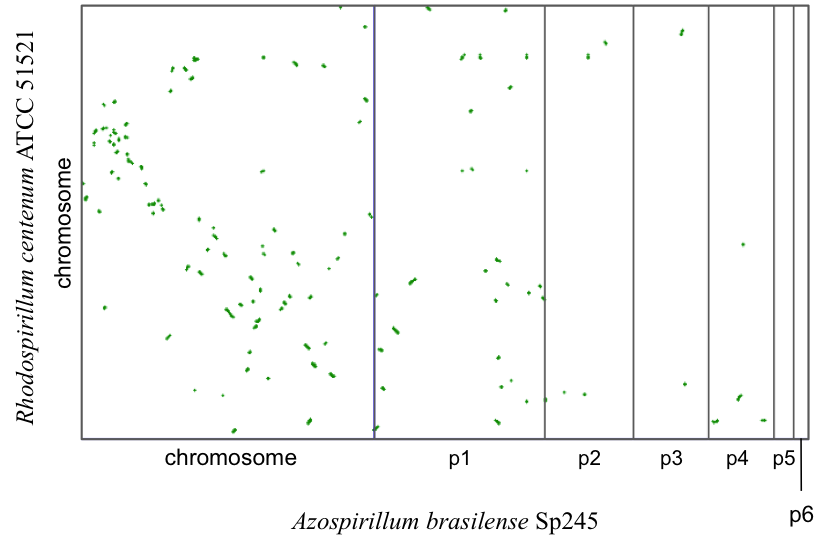
\includegraphics[width=0.7\textwidth]{./img/synteny/new/fig8_9.png}
	\caption[Synténie de \textit{Azospirillum} \textit{vs.} \textit{Rhodospirillum}]{Synténie d'\textit{Azospirillum brasilense} Sp245 (abscisse) \textit{vs.} \textit{Rhodospirillum centenum}  ATCC 51521 (ordonnée).}\label{figsyntazo}
\end{center}
\end{figure}   


\begin{table}[H]
\caption[Valeurs de l'indice synténique pour \textit{Azospirillum}]{Valeurs de l'indice synténique $S_{G}$ (éq. \ref{eqsynteny}) pour les réplicons du génome $G$ d'\textit{Azospirillum brasilense} Sp245 par rapport au génome $G_{ref}$ de \textit{Rhodospirillum centenum} ATCC 51521.}\label{tablesyntazo}
\begin{center}
	\begin{tabular}{c|c}
		$G \diagdown G_{ref}$ & $r^{ref}_{chr}$\\
		\hline
		$r_{chr}$ & 100\\
		$r_{AZOBRp1}$ & 63\\
		$r_{AZOBRp2}$ & 23\\
		$r_{AZOBRp3}$ & 9\\
		$r_{AZOBRp4}$ & 19\\
		 $r_{AZOBRp5}$ & 0\\
		$r_{AZOBRp6}$ & 0\\ 
	\end{tabular}
\end{center}
\end{table}  

Une synténie importante existe entre le chromosome de \textit{R. centenum} et le plus large plasmide d'\textit{A. brasilense}, renforçant le caractère de RECE d'AZOBRp1 (NC\_016594). Des synténies moins marquées existent aussi entre les plasmides additionnels et le chromosome indiquant de probables transferts latéraux. Ces résultats renforcent ceux présentés par Acosta-Cruz \textit{et al.} soutenant fortement la présence de RECE d'origine plasmidique dans le genre \textit{Azospirillum} \citep{Acosta-Cruz2012}. On peut supposer que, comme pour les Burkholdériales \citep{Passot2012}, les divers réplicons extra-chromosomiques d'\textit{Azospirillum} présentent des stades variables d'intégration dans le génome stable, observables par leur degré de synténie avec le génome de \textit{Rhodospirillum centenum} ATCC 51521.
    


\section{Génomes des Bétaprotéobactéries}\label{parburk}\label{parrals}
    La majorité des génomes multipartites référencés se trouve au sein des Burkholderiales, parmi les genres \textit{Burkholderia}, \textit{Ralstonia} et \textit{Cupriavidus}. Les génomes de \textit{B. multivorans} ATCC 17616 et de \textit{B. pseudomallei} sont comparés aux génomes de \textit{Bordetella bronchiseptica} 253, \textit{Ralstonia eutropha} H16 et de \textit{Polynucleobacter necessarius} STIR1 (Figure \ref{figsyntburk}). De même, le génome de \textit{Ralstonia eutropha} H16 est comparé à ceux de \textit{Bordetella bronchiseptica 253} et  \textit{Polynucleobacter necessarius} STIR1, ainsi qu'à celui de \textit{Janthinobacterium} sp. Marseille, une espèce appartenant à l'ordre des Burkholdériales et à la famille des Oxalobacteraceae \citep{hornung2013janthinobacterium}. Last est utilisé à cause de la grande taille des génomes comparés. \\
    Les \textit{Polynucleobacter} ont des génomes monopartites et sont membres, avec \textit{Burkholderia}, des Burkholderiaceae. \textit{Polynucleobacter necessarius} STIR1 est un endosymbiote d'\textit{Euplotes aediculatus} et possède un génome de petite taille (1.5 Mb) \citep{hahn2009emended}. Les autres espèces à génomes multipartites parmi les Burkholdériales sont des \textit{Ralstonia/Cupriavidus} de la famille des Ralstoniaceae, proche des Burkholderiaceae, et \textit{Variovorax}, membre des Comamonadaceae. Les Ralstoniaceae comportent plusieurs espèces à génome multipartite ou dont le genome comprend des mégaplasmides structurellement proches des RECE \citep{Passot2012}. \textit{Variovorax} est actuellement le seul exemple de génome multipartite chez les Comamonadaceae. Les espèces du genre \textit{Bordetella}, quant à elles, ont des génomes monopartites et font partie de la famille des Alcaligenaceae dans l'ordre des Burkholdériales. 


\begin{figure}[H]
\begin{center}
\hspace{-3cm}
	\begin{minipage}{0.5\textwidth}
		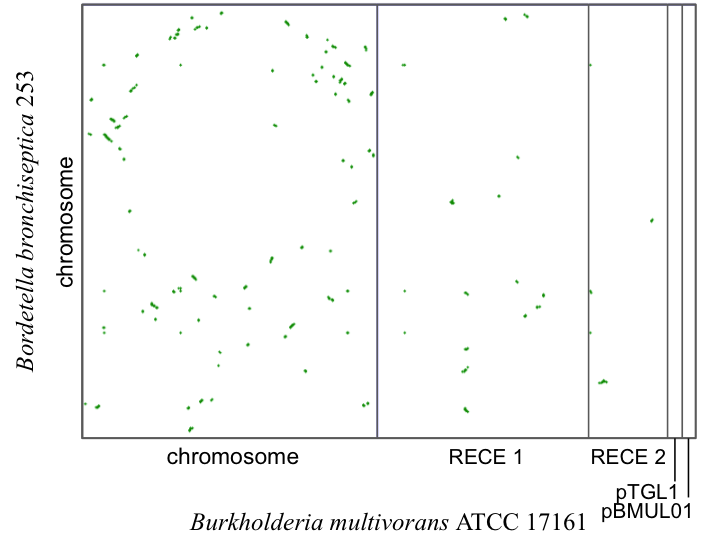
\includegraphics[width=1.1\textwidth]{./img/synteny/new/fig8_10a.png}
		\subcaption{\textit{B. multivorans} ATCC 17616 (abscisse) \textit{vs.} \textit{B. bronchiseptica} 253 (ordonnée).}\label{figsyntburk1}
	\end{minipage}
	\begin{minipage}{0.5\textwidth}
		\hspace{1cm}
		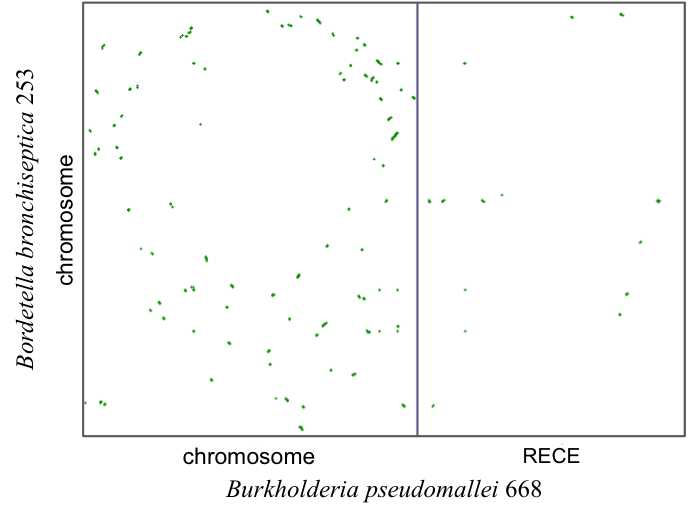
\includegraphics[width=1.1\textwidth]{./img/synteny/new/fig8_10b.png}
		\subcaption{\textit{B. pseudomallei} 668 (abscisse) \textit{vs.} \textit{B. bronchiseptica} 253 (ordonnée).}\label{figsyntburk2}
	\end{minipage}
\\
\vspace{0.5cm}
	\begin{minipage}{0.5\textwidth}
		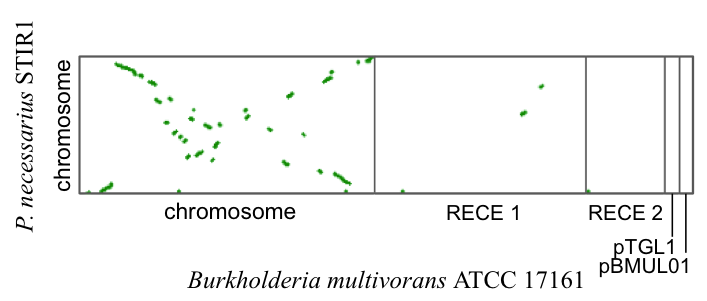
\includegraphics[width=1.1\textwidth]{./img/synteny/new/fig8_10c.png}
		\subcaption{\textit{B. multivorans} ATCC 17616 (abscisse) \textit{vs.} \textit{P. necessarius} STIR1 (ordonnée).}\label{figsyntburk3}
	\end{minipage}
\\
\vspace{0.5cm}
	\begin{minipage}{0.5\textwidth}
		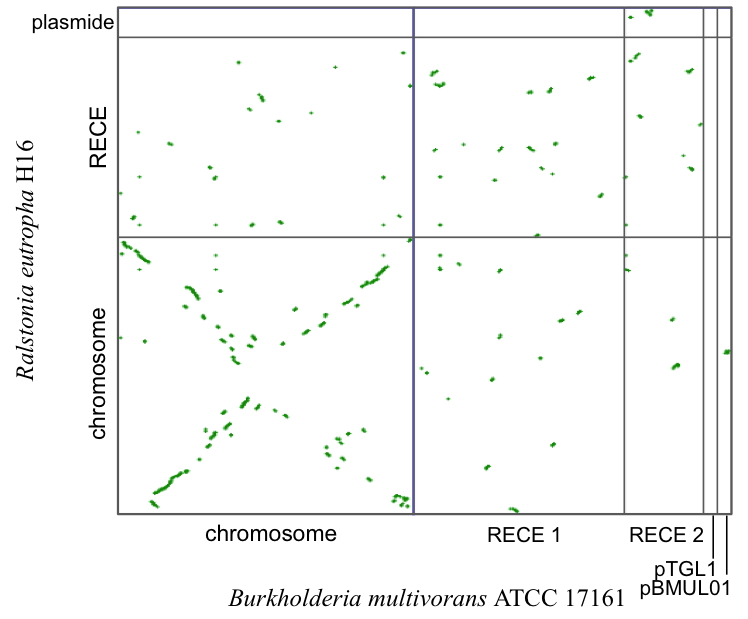
\includegraphics[width=1.1\textwidth]{./img/synteny/new/fig8_10d.png}
		\subcaption{\textit{B. multivorans} ATCC 17616 (abscisse) \textit{vs.} \textit{R. eutropha} H16 (ordonnée).}\label{figsyntburk4}
	\end{minipage}
\caption[Synténie de \textit{Burkholderia} \textit{vs.} autres Burkholderiales]{Synténie entre \textit{Burkholderia multivorans} ATCC 17616 et \textit{Burkholderia pseudomallei} 668 et \textit{Bordetella bronchiseptica} 253 (\ref{figsyntburk1} et \ref{figsyntburk2}, respectivement), et entre \textit{Burkholderia multivorans} ATCC 17616 et \textit{Polynucleobacter necessarius}  STIR1 (\ref{figsyntburk3}) et \textit{Ralstonia eutropha H16} (\ref{figsyntburk4}).} \label{figsyntburk}
\end{center}  
\end{figure}  

\begin{table}[H]
\caption[Valeurs de l'indice synténique pour \textit{Burkholderia}]{Valeurs de l'indice synténique $S_{G}$ (éq. \ref{eqsynteny}) pour les réplicons du génome $G$ de \textit{Burkholderia multivorans} ATCC 17616 par rapport aux génomes $G_{ref}$ de \textit{Bordetella bronchiseptica} 253 (\ref{tablesyntburk1}), \textit{Polynucleobacter necessarius} STIR1 (\ref{tablesyntburk3}) et \textit{Ralstonia eutropha} H16 (\ref{tablesyntburk3}), et pour les réplicons du génome $G$ de \textit{B. pseudomallei} 668 par rapport au génome $G_{ref}$ de \textit{B. bronchiseptica} 253 (\ref{tablesyntburk2}).}\label{tablesyntburk}
\begin{center}
	\begin{minipage}[t]{0.3\textwidth}
		\begin{tabular}{c|c}
			$G \diagdown G_{ref}$ & $r^{ref}_{chr}$\\
			\hline
			$r_{chr}$ & 100\\
			$ r_{RECE 1}$ & 21\\
			$r_{RECE 2}$ & 23\\
			$r_{pTGL1}$ & 0\\
			$r_{pBMUL01}$ & 0\\
		\end{tabular}
	\subcaption{\textit{B. multivorans} ATCC 17616 \textit{vs.} \textit{B. bronchiseptica} 253.}\label{tablesyntburk1}
	\end{minipage}
\hspace{1cm}
	\begin{minipage}[t]{0.3\textwidth}
		\begin{tabular}{c|c}
			$G \diagdown G_{ref}$ & $r^{ref}_{chr}$\\
			\hline
			$r_{chr}$ & 100\\
			$ r_{RECE}$ & 19\\
		\end{tabular}
	\subcaption{\textit{B. pseudomallei} 668 \textit{vs.} \textit{B. bronchiseptica} 253.}\label{tablesyntburk2}
	\end{minipage}
	\begin{minipage}[t]{0.3\textwidth}
		\begin{tabular}{c|c}
			$G \diagdown G_{ref}$ & $r^{ref}_{chr}$\\
			\hline
			$r_{chr}$ & 100\\
			$ r_{RECE 1}$ & 9\\
			$r_{RECE 2}$ & 3\\
			$r_{pTGL1}$ & 0\\
			$r_{pBMUL01}$ & 0\\
	\end{tabular}
	\subcaption{\textit{B. multivorans} ATCC 17616 \textit{vs.} \textit{P. necessarius} STIR1}\label{tablesyntburk3}
	\end{minipage}
	\begin{minipage}[t]{0.6\textwidth}
		\begin{tabular}{c|ccc}
			$G \diagdown G_{ref}$ & $r^{ref}_{chr}$ & $r^{ref}_{RECE}$ & $r^{ref}_{pGH1}$\\
			\hline
			$r_{chr}$ & 100 & 100 & n.a.\\
			$ r_{RECE 1}$ & 15 & 122 & n.a.\\
			$r_{RECE 2}$ & 9 & 167 & n.a.\\
			$r_{pTGL1}$ & 21 & 0 & n.a.\\
			$r_{pBMUL01}$ & 0 & 0 & n.a.\\
	\end{tabular}
	\subcaption{\textit{B. multivorans} ATCC 17616 \textit{vs.} \textit{R. eutropha} H16}\label{tablesyntburk4}
	\end{minipage}
\end{center}
\end{table}

Les espèces du genre \textit{Burkholderia} ont quasiment toutes des génomes multipartites. Il existe à ce jour une unique exception: le génome de \textit{B. rhizoxinica}. Selon les espèces de \textit{Burkholderia}, un ou deux RECE ont été identifiés. Ces réplicons sont généralement considérés comme étant issus de l'adaptation de mégaplasmides originels (\textit{cf.} Chapitre 2, \S \ref{chrIIess} et \S \ref{chrIIori}). Les réplicons des génomes de \textit{Burkholderia} possèdent un haut taux d'échange de gènes par TGH \citep{maida2014origin}. Les duplications géniques en résultant interviennent non seulement aux niveaux inter-chromosomique ou inter-plasmidique mais aussi entre chromosome et plasmide \citep{Passot2012}. Ces réarrangements sont proposés comme constituant un mécanisme fondamental dans l'évolution des génomes \citep{maida2014origin}. Enfin, il semble que des échanges inter-génomes ont lieu avec des espèces proches phylogéniquement \citep{maida2014origin}.\\	 
   Il est intéressant de constater que, malgré la nature hautement plastique des réplicons de \textit{Burkholderia}, seulement \textbf{\color{orange} une faible synténie existe entre les RECE de \textit{Burkholderia} et les chromosomes d'espèces proches phylogéniquement} en comparaison de la synténie existant entre chromosomes (Table \ref{tablesyntburk}). L'absence de ressemblance RECE/chromosome est confirmée par la comparaison avec le génome de \textit{Polynucleobacter necessarius} STIR1 (Figure \ref{figsyntburk3} et Table \ref{tablesyntburk3}). \textit{P. necessarius} possède un génome réduit de par son écologie endosymbiotique et son chromosome a donc tendance à n'abriter que des gènes de type chromosomique et essentiels. \\
Enfin, la comparaison de \textit{B. multivorans ATCC 17616} avec \textit{Ralstonia eutropha H16}  (Figure \ref{figsyntburk4} et Table \ref{tablesyntburk4}) montre une forte synténie entre les différents RECE, témoignant ainsi de leur origine commune. Les résultats mettent en évidence différents transferts entre RECE et chromosome spécifiques à \textit{Ralstonia} ou à \textit{Burkholderia}. \\
\\
De façon surprenante, \textbf{le RECE de \textit{R. eutropha} H16 possède de larges zones synténiques avec le chromosome de \textit{Bordetella bronchiseptica} 253} (Figure \ref{figsyntrals1} et Table \ref{tablesyntrals1}), et par contre, très peu avec les génomes de \textit{Janthinobacterium} sp. Marseille (Figure \ref{figsyntrals2} et Table \ref{tablesyntrals2}) et \textit{Polynucleobacter necessarius} STIR1 (Figure \ref{figsyntrals3} et Table \ref{figsyntrals3}), qui sont phylogéniquement plus proches de \textit{Ralstonia}. 


\begin{figure}[H]
\begin{center}
\hspace{-3cm}
	\begin{minipage}{0.5\textwidth}
		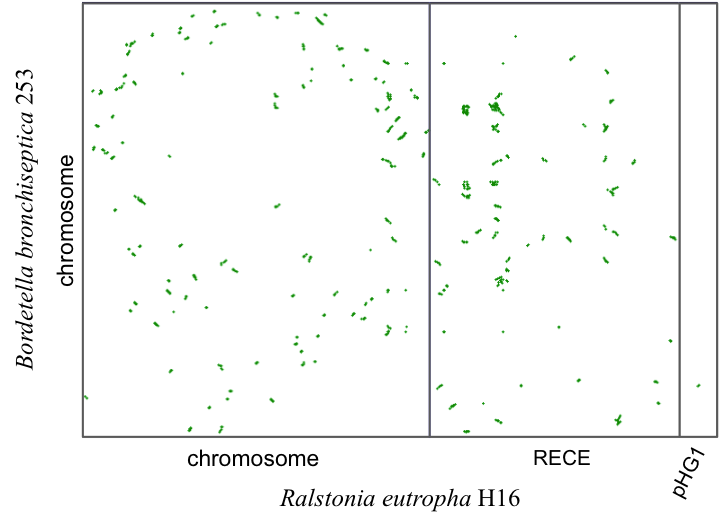
\includegraphics[width=\textwidth]{./img/synteny/new/fig8_11a.png}
		\subcaption{\textit{R. eutropha} H16 (abscisse) \textit{vs.} \textit{B. bronchiseptica} 253 (ordonnée).}\label{figsyntrals1}
	\end{minipage}
	\begin{minipage}{0.5\textwidth}
	\hspace{1cm}
		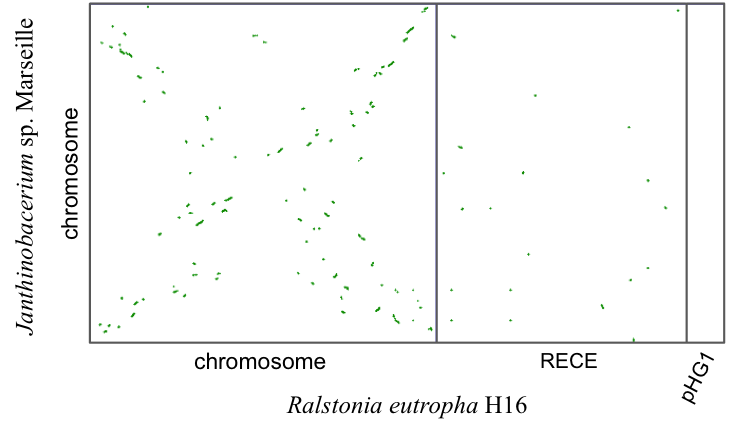
\includegraphics[width=1.1\textwidth]{./img/synteny/new/fig8_11b.png}
		\subcaption{\textit{R. eutropha} H16 (abscisse) \textit{vs.} \textit{Janthinobacterium} sp. Marseille (ordonnée).}\label{figsyntrals2}
	\end{minipage}
	\\   
	\begin{minipage}{0.5\textwidth}
		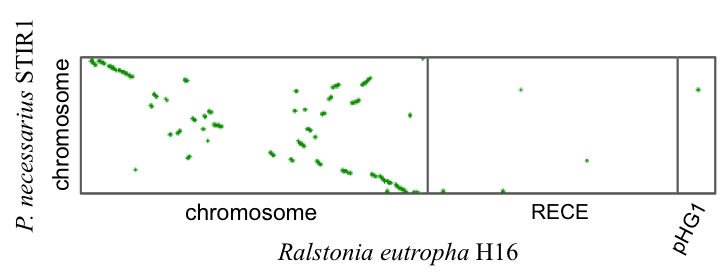
\includegraphics[width=\textwidth]{./img/synteny/new/fig8_11c.png}
		\subcaption{\textit{R. eutropha} H16 (abscisse) \textit{vs.} \textit{P. necessarius} STIR1 (ordonnée).}\label{figsyntrals3}
	\end{minipage}
\caption[Synténie de \textit{Ralstonia} \textit{vs.} autres Burkholderiales]{Synténie du génome de \textit{Ralstonia eutropha H16} avec les génomes monopartites de \textit{Bordetella bronchiseptica 253} (\ref{figsyntrals1}), \textit{Janthinobacterium} sp. strain Marseille (\ref{figsyntrals2}), et \textit{Polynucleobacter necessarius} STIR1 (\ref{figsyntrals3}).}\label{figsyntrals}
\end{center} 
\end{figure}  

\begin{table}[H]
   \caption[Valeurs de l'indice synténique pour \textit{Ralstonia}]{Valeurs de l'indice synténique $S_{G}$ (éq. \ref{eqsynteny}) pour les différents réplicons du génome $G$ de \textit{Ralstonia eutropha} H16 par rapport aux génomes $G_{ref}$ de \textit{Bordetella bronchiseptica} 253 (\ref{tablesyntrals1}), \textit{Janthinobacterium} sp. Marseille (\ref{tablesyntrals2}) et \textit{Polynucleobacter necessarius} STIR1 (\ref{tablesyntrals3}).}\label{tablesyntrals}
   \begin{center}
   \begin{minipage}[t]{0.3\textwidth}
   \begin{tabular}{c|c}
   $G \diagdown G_{ref}$ & $r^{ref}_{chr}$\\
   \hline
    $r_{chr}$ & 100\\
   $ r_{RECE}$ & 71\\
   $r_{pHG1}$ & 9\\
   \end{tabular}
   \subcaption{\textit{R. eutropha} H16 \textit{vs.} \textit{B. bronchiseptica} 253.}\label{tablesyntrals1}
   \end{minipage}
   \hspace{1cm}
   \begin{minipage}[t]{0.3\textwidth}
   \begin{tabular}{c|c}
   $G \diagdown G_{ref}$ & $r^{ref}_{chr}$\\
   \hline
   $r_{chr}$ & 100\\
   $ r_{RECE}$ & 17\\
   $r_{pHG1}$ & 0\\
   \end{tabular}
   \subcaption{\textit{R. eutropha} H16 \textit{vs.} \textit{Janthinobacterium} sp. Marseille.}\label{tablesyntrals2}
   \end{minipage}
   \begin{minipage}[t]{0.3\textwidth}
   \begin{tabular}{c|c}
   $G \diagdown G_{ref}$ & $r^{ref}_{chr}$\\
   \hline
   $r_{chr}$ & 100\\
   $ r_{RECE}$ & 4\\
   $r_{pHG1}$ & 6\\
   \end{tabular}
   \subcaption{\textit{R. eutropha} H16 \textit{vs.} \textit{P. necessarius} STIR1.}\label{tablesyntrals3}
   \end{minipage}
   \end{center}
\end{table}

Des résultats similaires sont obtenus en comparant les génomes d'espèces additionnelles de \textit{Bordetella} et de \textit{Ralstonia/Cupriavidus} (résultats non montrés). Le fait cependant qu'une faible synténie est partagée entre le RECE de \textit{R. eutropha} H16 et les génomes monopartites de \textit{Janthinobacterium} et \textit{Polynucleobacter} indiquerait un événement génomique spécifique au genre \textit{Bordetella}. \textbf{\color{orange} En rapprochant la valeur de l'indice de synténie obtenue entre le RECE de \textit{R. eutropha strain} H16 et le chromosome de \textit{B. bronchiseptica} 253 à celles obtenues pour le génome de \textit{Mesorhizobium}, on peut penser que le génome ancestral des \textit{Bordetella} a intégré une partie des gènes du réplicon ancestral des RECE de \textit{Ralstonia/Cupriavidus}.} Cette hypothèse est à confirmer par une étude plus fine des génomes des \textit{Bordetella}.  
     

\section{Génomes des Gamma-protéobactéries}\label{parvibr}
   Les génomes multipartites des Gammaprotéobactéries sont trouvés chez tous les membres (décrits à ce jour) des Vibrionales et chez deux \textit{Pseudoalteromonas}, parmi les Alteromonadales: \textit{Pseudoalteromonas haloplanktis} TAC125 et \textit{Pseudoalteromonas} sp. SM9913. Le génome d'\textit{Aliivibrio fisheri} ES114 (Vibrionaceae, Vibrionales) est comparé aux génomes de \textit{Vibrio cholerae} O1 biovar El Tor N16961  (Vibrionaceae, Vibrionales), \textit{Photobacterium profundum} SS9 (Photobacteriaceae,Vibrionales), \textit{Shewanella amazonensis} SB2B (Shewanellaceae), et \textit{Pseudoalteromonas haloplanktis} TAC125 (Alteromonadaceae). En raison de la taille des génomes, Last est utilisé.
    
\begin{table}[H]
\begin{center}
\caption[Valeurs de l'indice synténique pour \textit{Aliivibrio}]{Valeurs de l'indice synténique $S_{G}$ (éq. \ref{eqsynteny}) pour les réplicons du génome $G$ d'\textit{Aliivibrio fischeri} ES114 par rapport aux génomes $G_{ref}$ de \textit{Vibrio cholerae} O1 biovar El Tor N16961 (\ref{tablesyntvib1}), \textit{Shewanella amazonensis} SB2B (\ref{tablesyntvib2}, génome monopartite), \textit{Pseudoalteromonas haloplanktis} TAC125 (\ref{tablesyntvib3}) et \textit{Photobacterium profundum} SS9 (\ref{tablesyntvib4}), et pour les réplicons de \textit{Vibrio cholerae} O1 biovar El Tor N16961 par rapport au génome de \textit{Photobacterium profundum} SS9 (\ref{tablesyntvib5}).} \label{tablesyntsphing}
   \begin{minipage}[t]{0.3\textwidth}
   \subcaption{\textit{A. fischeri} ES114 \textit{vs.} \textit{V. cholerae} N16961.}\label{tablesyntvib1}
   	\begin{tabular}{c|cc}
    		$G \diagdown G_{ref}$ & $r^{ref}_{chr}$ & $r^{ref}_{RECE} $\\
   		\hline
   		$r_{chr}$ & 100 & 100\\
  		 $ r_{RECE}$ & 10 & 544\\
   	\end{tabular}
   \end{minipage}
   \hspace{1cm}
   \begin{minipage}[t]{0.3\textwidth}
   \subcaption{\textit{A. fischeri} ES114 \textit{vs.} \textit{Shewanella amazonensis} SB2B.}\label{tablesyntvib2}
   	\begin{tabular}{c|c}
   		$G \diagdown G_{ref}$ & $r^{ref}_{chr}$\\
   		\hline
    		$r_{chr}$ & 100\\
   		$ r_{RECE}$ & 1\\
   	\end{tabular}
   \end{minipage}
   \\
   \begin{minipage}[t]{0.3\textwidth}
   \hspace{-1cm}
   \subcaption{\textit{A. fischeri} ES114 \textit{vs.} \textit{P. haloplanktis} TAC125.}\label{tablesyntvib3}
   	\begin{tabular}{c|cc}
   		$G \diagdown G_{ref}$ & $r^{ref}_{chr}$ & $r^{ref}_{RECE} $\\
   		\hline
    		$r_{chr}$ & 100 & 100\\
   		$ r_{RECE}$ & 6 & 42\\
   	\end{tabular}
   \end{minipage}
   \begin{minipage}[t]{0.3\textwidth}
   \subcaption{\textit{A. fischeri} ES114 \textit{vs.} \textit{P. profundum} SS9.}\label{tablesyntvib4}
   	\begin{tabular}{c|ccc}
   		$G \diagdown G_{ref}$ & $r^{ref}_{chr}$ & $r^{ref}_{RECE}$ & $r^{ref}_{pPBPR1}$\\
   		\hline
    		$r_{chr}$ & 100 & 100 & n.a.\\
   		$r_{RECE}$ & 11 & 226 & n.a.\\
   		\end{tabular}
   \end{minipage}
   \\
 	\begin{minipage}[t]{0.4\textwidth}
   \subcaption{\textit{V. cholerae} N16961 \textit{vs.} \textit{P. profundum} SS9.}\label{tablesyntvib5}
   	\begin{tabular}{c|ccc}
   		$G \diagdown G_{ref}$ & $r^{ref}_{chr}$ & $r^{ref}_{RECE}$ & $r^{ref}_{pPBPR1}$\\
   		\hline
    		$r_{chr}$ & 100 & 100 & n.a.\\
   		$r_{RECE}$ & 6 & 311 & n.a.\\
   	\end{tabular}
	\end{minipage}  
   \end{center}
\end{table}     

  Les résultats pour les génomes de \textit{Vibrionales} (Figures \ref{figsyntvib1}, \ref{figsyntvib4} et \ref{figsyntvib5}) sont similaires au cas des génomes des \textit{Burkholderia} (Figure \ref{figsyntburk4}). Un signal synténique fort témoigne de l'origine commune de leurs RECE (Tables \ref{tablesyntvib1}, \ref{tablesyntvib4} et \ref{tablesyntvib5}), mais avec des transferts RECE/chromosome propres à chaque lignée. L'étude de \textit{Vibrio} avec \textit{Shewanella}, dont le génome est monopartite, montre une synténie quasiment nulle entre le RECE et le chromosome (Figure \ref{figsyntvib2} et Table \ref{tablesyntvib2}). Enfin, l'étude de \textit{Vibrio} avec \textit{Pseudoalteromonas} (Figure \ref{figsyntvib3} et Table \ref{tablesyntvib3}) ne détecte aucune synténie entre les deux RECE suggérant que ceux-ci sont issus d'événements évolutifs distincts.
  
\begin{figure}[H]
\begin{center}
\hspace{-3cm}
	\begin{minipage}{0.5\textwidth}
   		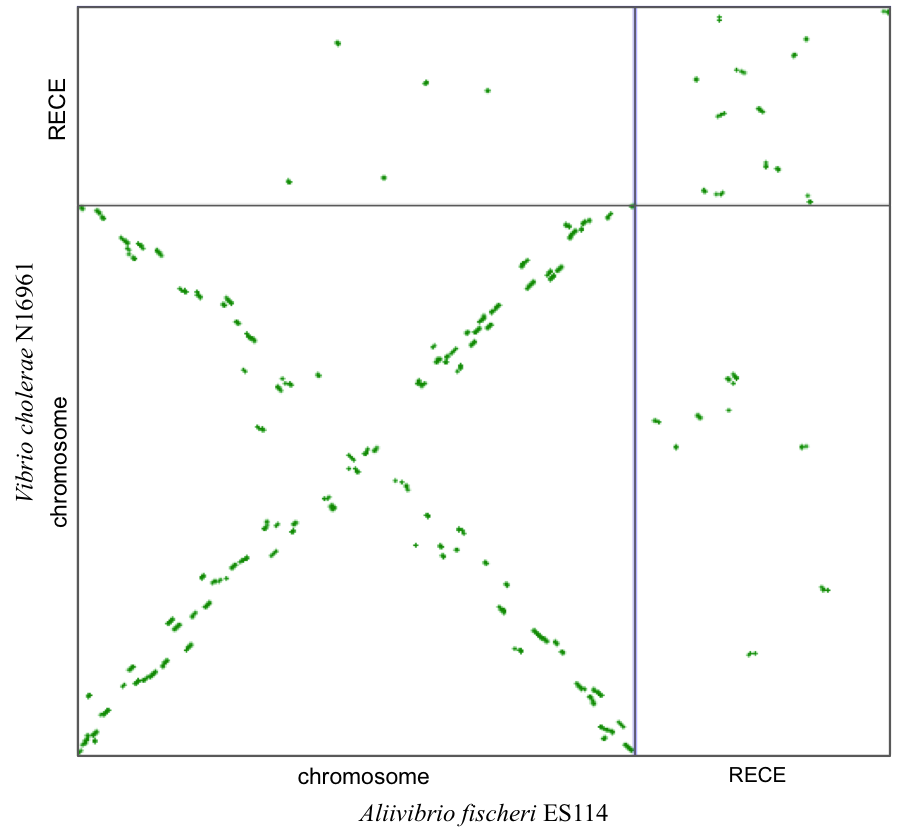
\includegraphics[width=\textwidth]{./img/synteny/new/fig8_12a.png}
   		\subcaption{\textit{A. fischeri} ES114 (abscisse) \textit{vs.} \textit{V. cholerae} N16961 (ordonnée).}\label{figsyntvib1}
	\end{minipage}
  	\begin{minipage}{0.5\textwidth}
  		\hspace{1cm}
   		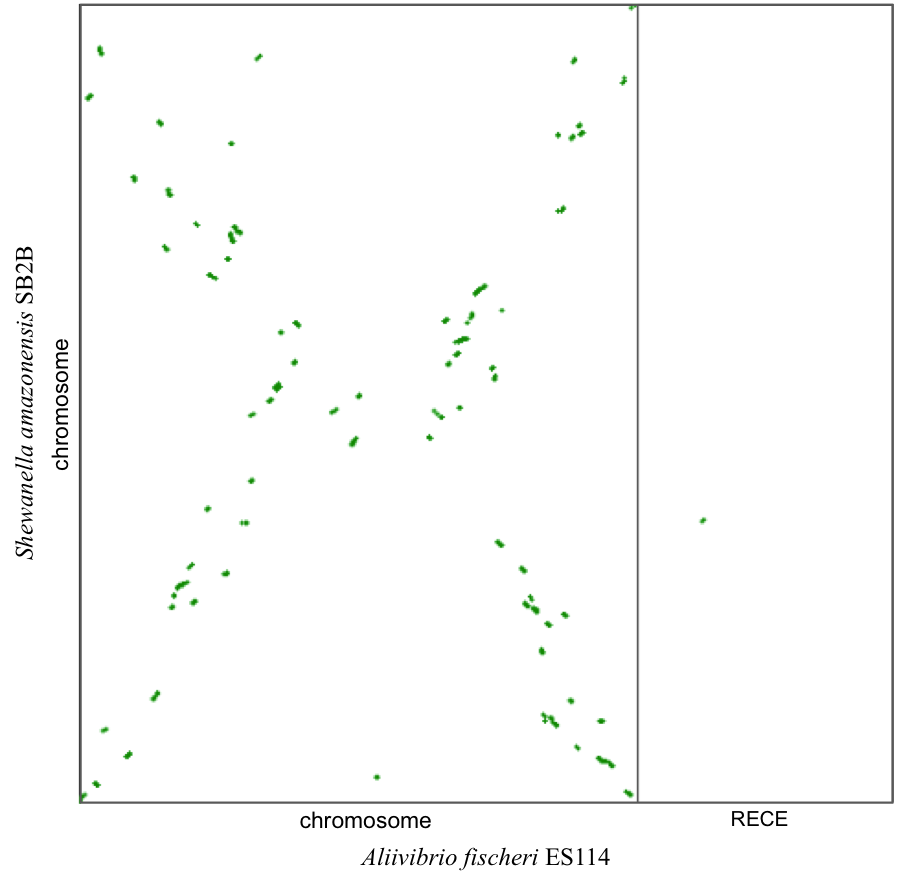
\includegraphics[width=1.1\textwidth]{./img/synteny/new/fig8_12b.png}
   		\subcaption{\textit{A. fischeri} ES114 (abscisse) \textit{vs.} \textit{Shewanella amazonensis} SB2B (ordonnée).}\label{figsyntvib2}
	\end{minipage}
\\
\hspace{-3cm}
	\begin{minipage}{0.5\textwidth}
   		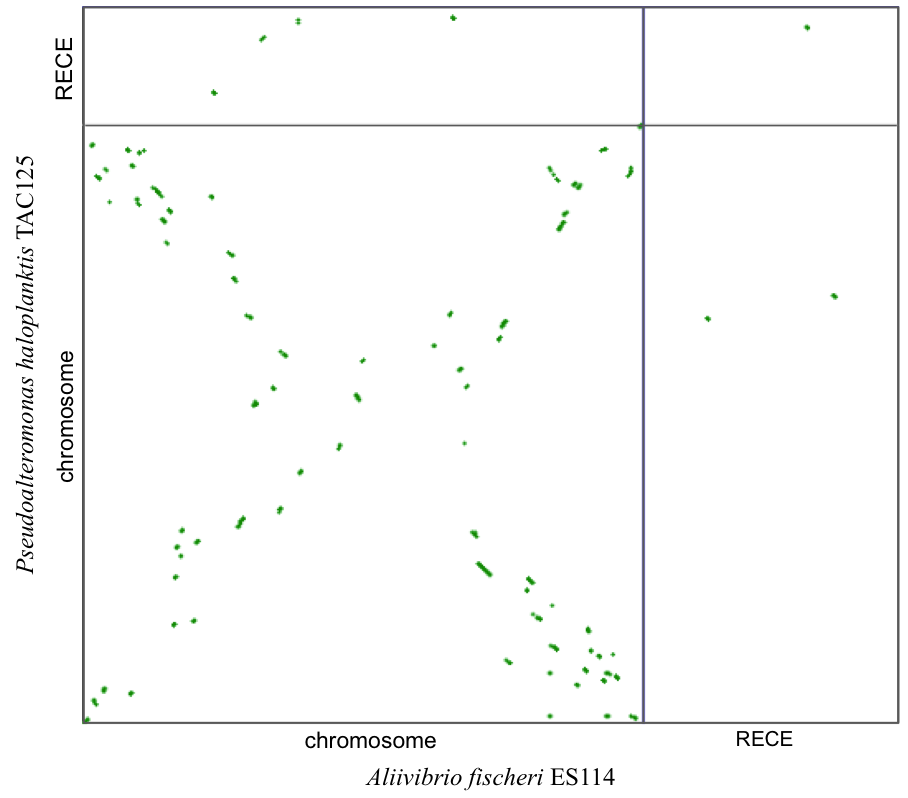
\includegraphics[width=\textwidth]{./img/synteny/new/fig8_12c.png}
   		\subcaption{\textit{A. fischeri} ES114 (abscisse) \textit{vs.} \textit{P. haloplanktis} TAC125 (ordonnée).}\label{figsyntvib3}
	\end{minipage}
	\begin{minipage}{0.5\textwidth}
   		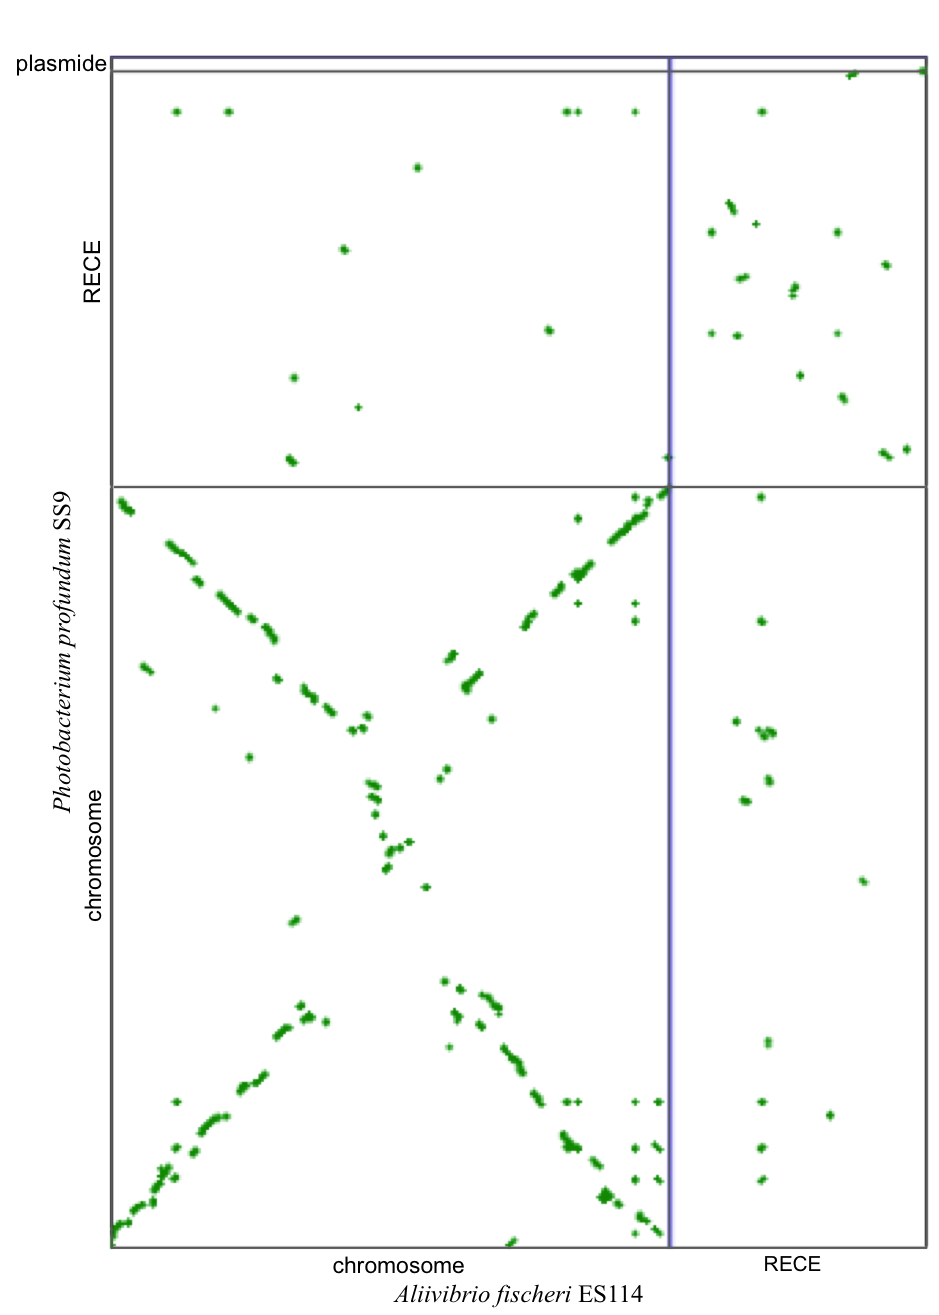
\includegraphics[width=\textwidth]{./img/synteny/new/fig8_12d.png}
   		\subcaption{\textit{A. fischeri} ES114 (abscisse) \textit{vs.} \textit{P. profundum} SS9 (ordonnée).}\label{figsyntvib4}
	\end{minipage}
\end{center}
\end{figure} 

%\iffalse
\begin{figure}[H]
\centering
	\begin{minipage}{0.5\textwidth}
   		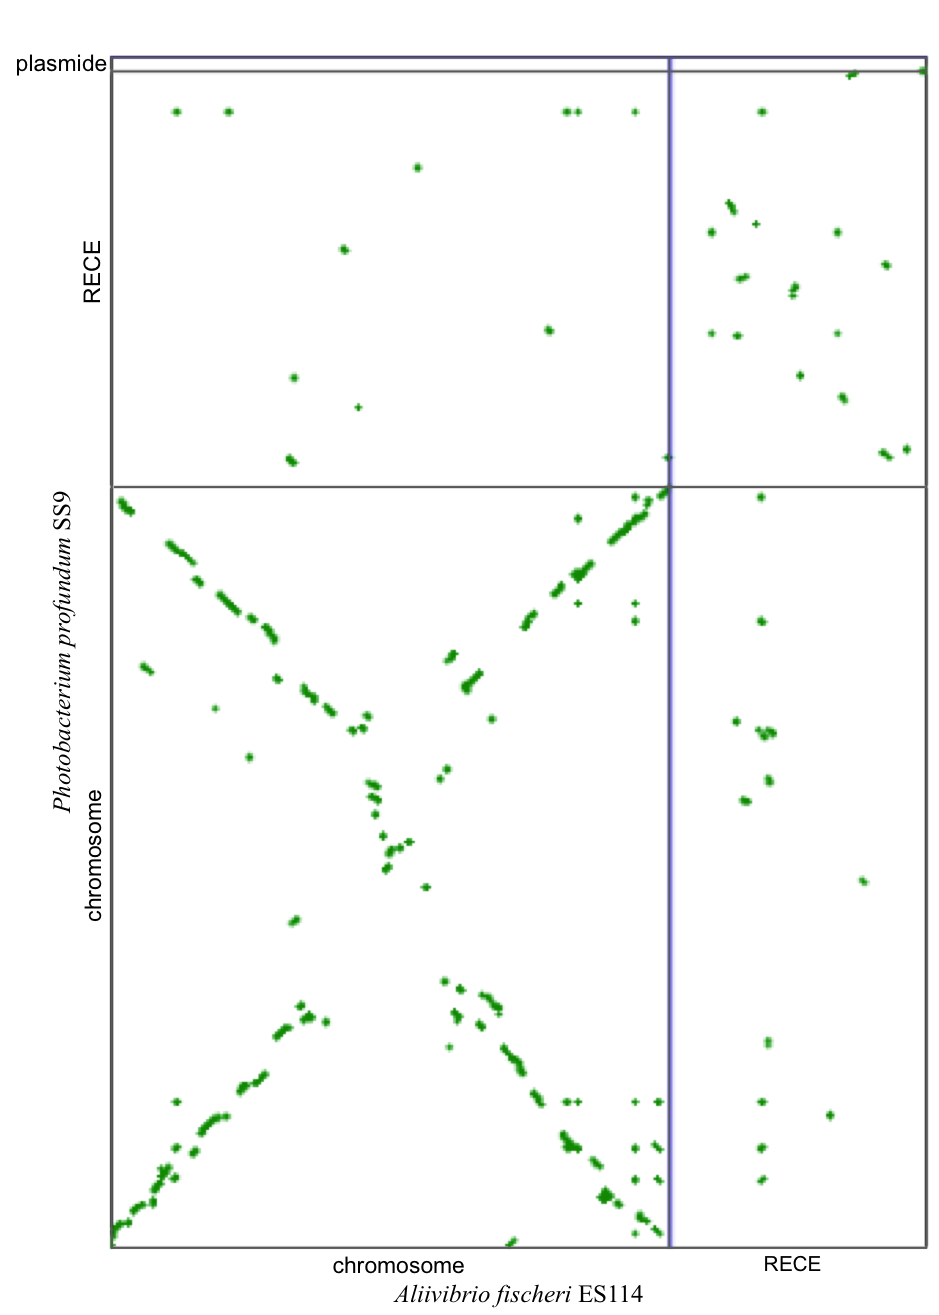
\includegraphics[width=\textwidth]{./img/synteny/new/fig8_12d.png}
   		\subcaption{\textit{V. cholerae} N16961 (abscisse) \textit{vs.} \textit{P. profundum} SS9 (ordonnée).}\label{figsyntvib5}
    \end{minipage} 
\end{figure}      
      
\captionof{figure}[Synténie de \textit{Aliivibrio} \textit{vs.} gammaprotéobactéries proches]{Synténie entre \textit{Allivibrio fischeri} ES114 et \textit{Vibrio cholerae} O1 biovar El Tor N16961 (\ref{figsyntvib1}), \textit{Shewanella amazonensis} SB2B (\ref{figsyntvib2}), \textit{Pseudoalteromonas haloplanktis} TAC125 (\ref{figsyntvib3}) et \textit{Photobacterium profundum} SS9 (\ref{figsyntvib4}), et  \textit{Vibrio cholerae} O1 biovar El Tor N16961 et \textit{Photobacterium profundum} SS9 (\ref{figsyntvib5}).}\label{figsyntvib}
\vspace{1cm}
Curieusement, \textbf{Il existe une synténie relativement plus forte entre les chromosomes et les RECE de \textit{A. fisherii} et \textit{P. profundum} par comparaison à \textit{V. cholerae}} (Figures \ref{figsyntvib4} et \ref{figsyntvib5}), bien qu'ils soient phylogéniquement moins proches qu'\textit{A. fisherii} et \textit{V. cholerae}. Il semble donc que des phénomènes de transfert entre les chromosomes et les RECE des \textit{Aliivibrio} et \textit{Photobacterium} ont eu lieu récemment.

\newpage
\section{Génomes des Cyanobactéries}
	Deux génomes multipartites sont actuellement référencés chez les Cyanobactéries et appartiennent à deux ordres différents.     

\subsection{Analyse des Nostocales}\label{paranab}
   Le génome multipartite d'\textit{Anabaena} sp. 90 est comparé au génome monopartite de \textit{Anabaena} sp. PCC 7120 (Figure \ref{figsyntcyanothece} et Table \ref{tablesyntanabaena}). \textit{blastn} est utilisé. 

\begin{figure}[H]
   \begin{center}
   	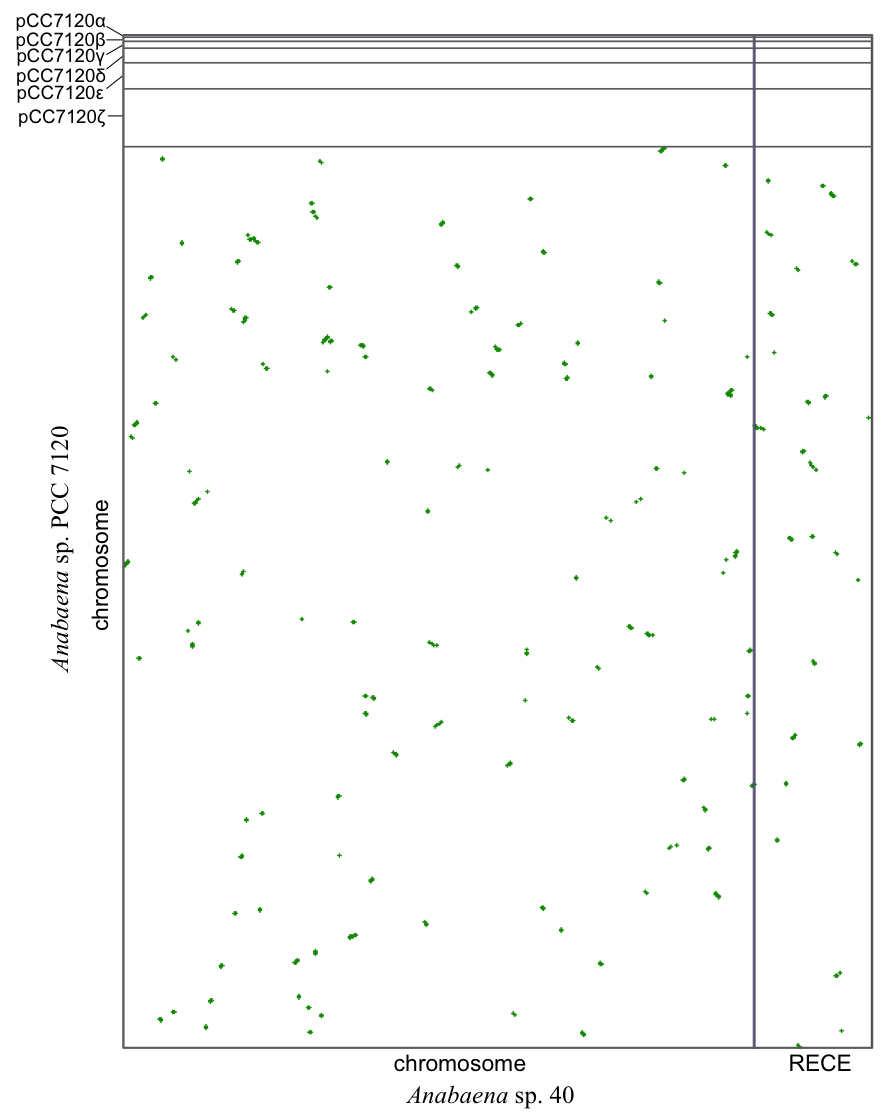
\includegraphics[width=0.8\textwidth]{./img/synteny/new/fig8_13.png}
   	\caption[Synténie entre espèces multi-/monopartite d'\textit{Anabaena}]{Synténie d'\textit{Anabaena} sp. 90 (ordonnée) \textit{vs.} \textit{Anabaena} sp. PCC 7120 (abscisse).}\label{figsyntanabaena}
   \end{center}
\end{figure}   

\begin{table}[H]
	\hspace{-1cm}
	\begin{minipage}{\textwidth}
   \begin{center}
			\caption[Valeurs de l'indice synténique pour \textit{Anabaena}]{Valeurs de l'indice synténique de synténie $S_{G}$ (éq. \ref{eqsynteny}) pour les réplicons du génome $G$ d'\textit{Anabaena} sp. 90 par rapport au génome $G_{ref}$ d'\textit{Anabaena} sp. PCC 7120}\label{tablesyntanabaena}
   		\begin{tabular}{c|cccccccc}
   			$G \diagdown G_{ref}$ & $r^{ref}_{chr}$ & $r^{ref}_{pCC7120\alpha}$ & $r^{ref}_{pCC7120\alpha}$ & $r^{ref}_{pCC7120\beta}$ & 
   $r^{ref}_{pCC7120\gamma}$ & $r^{ref}_{pCC7120\delta}$ & $r^{ref}_{pCC7120\epsilon}$
    & $r^{ref}_{pCC7120\zeta}$\\
   			\hline
   			$r_{chr}$ & 100 & n.a. & n.a. & n.a. & n.a. & n.a. & n.a. & n.a.\\
   			$ r_{RECE}$ & 120 & n.a. & n.a. & n.a. & n.a. & n.a. & n.a. & n.a.\\
   		\end{tabular}
   \end{center}
   \end{minipage}
\end{table}

Comme pour le génome multipartite d'\textit{Asticcacaulis}, les zones de synténie entre le RECE d'\textit{Anabaena} sp. 90 et le chromosome d'\textit{Anabaena} sp. PCC 7120 sont relativement plus grandes qu'entre les chromosomes de ces deux espèces. Par ailleurs, le RECE d'\textit{Anabaena} sp. 90 ne possède aucune région de synténie avec les plasmides d'\textit{Anabaena sp. PCC 7120}. Enfin, malgré un signal synténique plus faible, \textbf{des résultats similaires ont été obtenus en comparant \textit{Anabanea} avec des génomes monopartites de cyanobactéries plus distantes phylogéniquement: \textit{Trichodesmium erythraeum} IMS101 et \textit{Synechococcus elongatus} PCC 7942} (résultats non montrés).
 

\subsection{Analyse des Chroococcales}\label{parcyan}
	 Le génome multipartite de \textit{Cyanothece} sp. ATCC 51142 est comparé au génome monopartite de \textit{Cyanothece} sp. PCC 8801 (Figure \ref{figsyntcyanothece} et Table \ref{tablesyntcyanothece}). \textit{blastn} est utilisé. 	

\begin{figure}[H]
   \begin{center}
   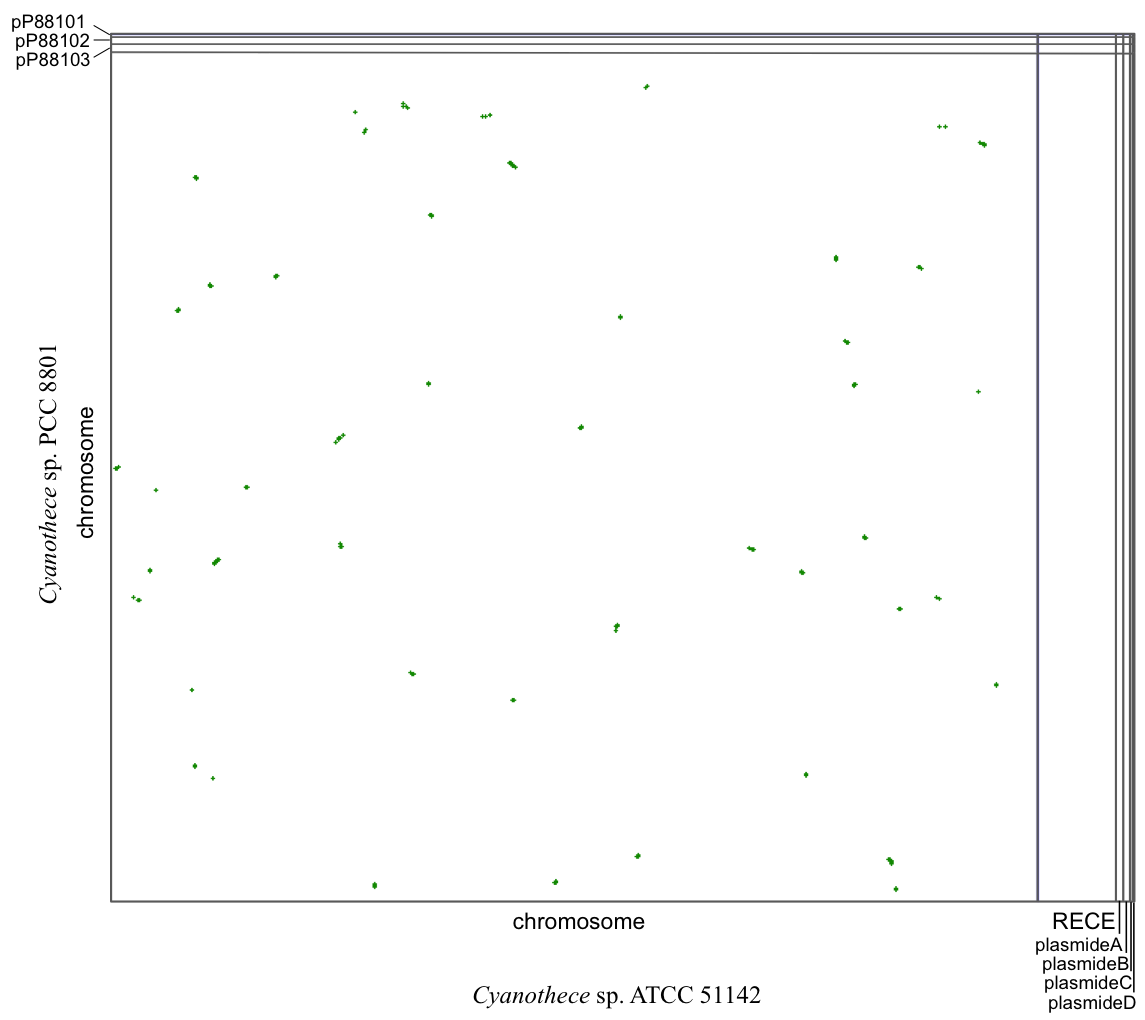
\includegraphics[width=0.6\textwidth]{./img/synteny/new/fig8_14.png}
   \caption[Synténie entre espèces multi-/monopartite de \textit{Cyanothece}]{Synténie entre \textit{Cyanothece} sp. ATCC 51142 (ordonnée) et \textit{Cyanothece} sp. PCC 8801 (abscisse).}\label{figsyntcyanothece}
   \end{center}
\end{figure}   

\begin{table}[H]
	\hspace{-1cm}
	\begin{minipage}{\textwidth}
	\begin{center}
	\caption[Valeurs de l'indice synténique pour \textit{Cyanothece}]{Valeurs de l'indice synténique de synténie $S_{G}$ (éq. \ref{eqsynteny}) pour les réplicons du génome $G$ de \textit{Cyanothece} sp. ATCC 51142 par rapport au génome $G_{ref}$ de \textit{Cyanothece} sp. PCC 8801.}\label{tablesyntcyanothece}
   \begin{tabular}{c|cccc}
    $G \diagdown G_{ref}$ & $r^{ref}_{chr}$ & $r^{ref}_{pP880101}$ & $r^{ref}_{pP880102}$ & $r^{ref}_{pP880103}$\\
   \hline
   $r_{chr}$ & 100 & n.a. & n.a. & n.a. \\
   $ r_{RECE}$ & 0 & n.a. & n.a. & n.a. \\
   $r_{plasmide A}$&0 & n.a. & n.a. & n.a. \\
   $r_{plasmide B}$&0 & n.a. & n.a. & n.a.\\
   $r^{ref}_{plasmide C}$&0 & n.a. & n.a. & n.a.\\
   $r^{ref}_{plasmide D}$&0 & n.a. & n.a. & n.a.\\
   \end{tabular}
   \end{center}
   \end{minipage}
   \end{table}	
   
Aucune synténie n'est detectée entre le RECE de \textit{Cyanothece} sp. ATCC 51142 et le chromosome de \textit{Cyanothece} sp. PCC 8801 ou ses plasmides. La synténie partagée entre les deux chromosomes est relativement faible pour des génomes de bactéries du même genre. Des résultats similaires ont été obtenus en utilisant d'autres génomes de \textit{Cyanothece} sp. et \textit{Acaryochloris marina} MBIC11017 (résultats non montrés). Les signaux synténiques étant très faibles, il est difficile de comparer les génomes de \textit{Cyanothece} avec des génomes monopartites d'espèces plus distantes.



\section{Génomes des Bacteroidetes}\label{parprev}
	Deux génomes multipartites ont été identifiés parmi les \textit{Prevotella}, espèces appartenant aux Bacteroidia, un des ordres de Bacteroidetes. Le génome multipartite de \textit{P. intermedia} 17 a été comparé aux génomes monopartites de \textit{P. ruminicola} 23, de \textit{P. denticola} F0289 et de \textit{Bacteroides fragilis} YCH46 (Figure \ref{figsyntprev} et Table \ref{tablesyntprev}). \textit{blastn} a été utilisé. \textbf{Étrangement, le chromosome (présence de \textit{dnaA}) de \textit{P. intermedia} 17 est le plus petit des réplicons essentiels du génome}. 

\begin{table}[H]
   \begin{center}
   \hspace{-1.5cm}
   \caption[Valeurs de l'indice synténique pour \textit{Prevotella}]{Valeurs de l'indice synténique $S_{G}$ (éq. \ref{eqsynteny}) pour les réplicons du génome $G$ de \textit{Prevotella intermedia} 17 par rapport aux génomes $G_{ref}$ de \textit{P. ruminicola} 23 (\ref{tablesyntprev1}), \textit{P. denticola} F0289 (\ref{tablesyntprev2}) et \textit{Bacteroides fragilis} YCH46 (\ref{tablesyntprev3}).}\label{tablesyntprev}
   \begin{minipage}[t]{0.3\textwidth}
   \subcaption{\textit{P. intermedia} 17 \textit{vs.} \textit{P. ruminicola} 23.}\label{tablesyntprev1}
   	\begin{tabular}{c|c}
   		$G \diagdown G_{ref}$ & $r^{ref}_{chr}$\\
   		\hline
   		$r_{chr}$ & 100\\
   		$ r_{RECE}$ & 153\\
   	\end{tabular}
   \end{minipage}
   \hspace{0.5cm}
   \begin{minipage}[t]{0.3\textwidth}
   \subcaption{\textit{P. intermedia} 17 \textit{vs.} \textit{P. denticola} F0289.}\label{tablesyntprev2}
   	\begin{tabular}{c|c}
   		$G \diagdown G_{ref}$ & $r^{ref}_{chr}$\\
   		\hline
   		$r_{chr}$ & 100\\
   		$ r_{RECE}$ & 178\\
	   \end{tabular}
   \end{minipage}
   \hspace{0.3cm}
   \begin{minipage}[t]{0.3\textwidth}
   \subcaption{\textit{P. intermedia} 17 \textit{vs.} \textit{B. fragilis} YCH46.}\label{tablesyntprev3}
   	\begin{tabular}{c|cc}
   		$G \diagdown G_{ref}$ & $r^{ref}_{chr}$ & $r^{ref}_{pBFY46}$\\
   		\hline
   		$r_{chr}$ & 100 & n.a.\\
   		$ r_{RECE}$ & 158 & n.a.\\
   		\end{tabular}
   		\end{minipage}
   \end{center}
   \end{table}
   
	Dans cette configuration, le RECE de \textit{P. intermedia} 17 présente la plus forte synténie avec les chromosomes des génomes monopartites comparés. Au contraire, le réplicon annoté dans RefSeq comme chromosome chez \textit{P. intermedia} 17 se rapproche davantage des RECE décrits précédemment que des chromosomes authentiques (\textit{i.e.}, ressemblant plus aux chromosomes). La  synténie de ce ``chromosome-RECE" de \textit{P. intermedia} 17 s'avère cependant relativement importante en comparaison aux chromosomes et, de plus, \textbf{est conservée pour des génomes plus éloignés appartenant aux Bacteroidetes}. Toutefois, une interprétation définitive n'est pas possible compte tenu du peu de zones de synténie conservées entre génomes du même genre (\textit{Prevotella}). 
     
\begin{figure}[H]
   \begin{center}
   \vspace{-0.5cm}
   \hspace{-2cm}
   \begin{minipage}{0.5\textwidth}
   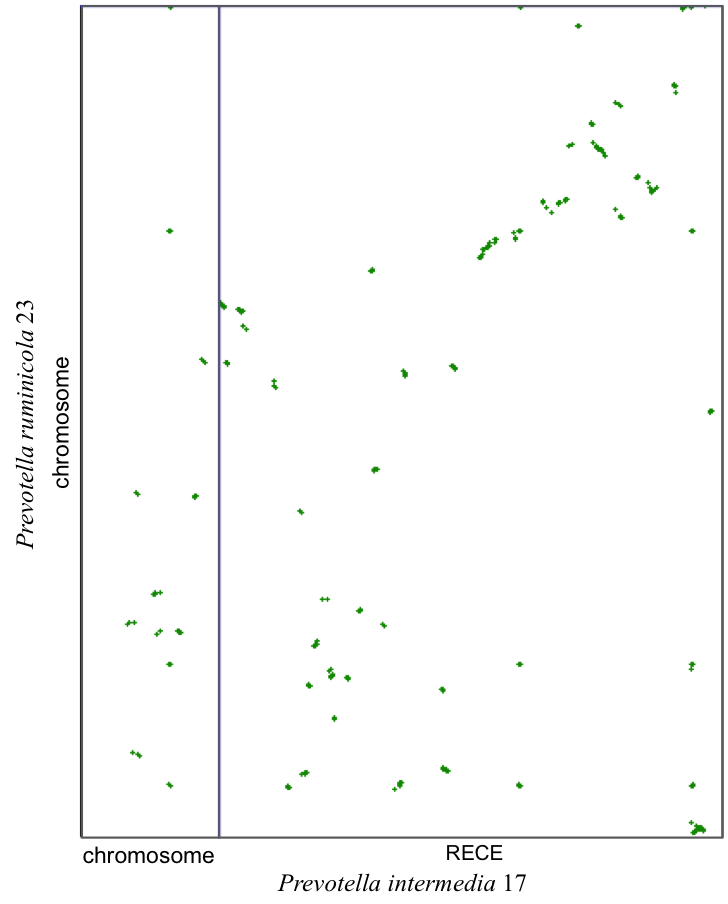
\includegraphics[width=1.1\textwidth]{./img/synteny/new/fig8_15a.png}
   \subcaption{\mbox{\textit{P. intermedia} 17 (abscisse) \textit{vs.} \textit{P. ruminicola} 23 (ordonnée).}}\label{figsyntprev1}
    \end{minipage}
  \begin{minipage}{0.5\textwidth}
  \hspace{1cm}
   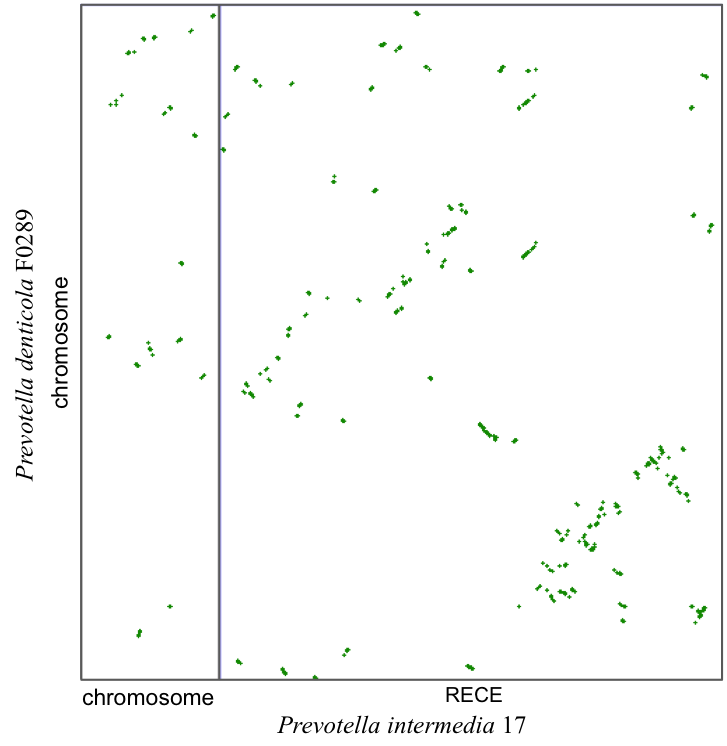
\includegraphics[width=1.1\textwidth]{./img/synteny/new/fig8_15b.png}
   \hspace{2cm}
   \subcaption{\textit{P. intermedia} 17 (abscisse) \textit{vs.} \textit{P. denticola} F0289 (ordonnée).}\label{figsyntprev2}
    \end{minipage}
    \\
    \begin{minipage}{0.5\textwidth}
   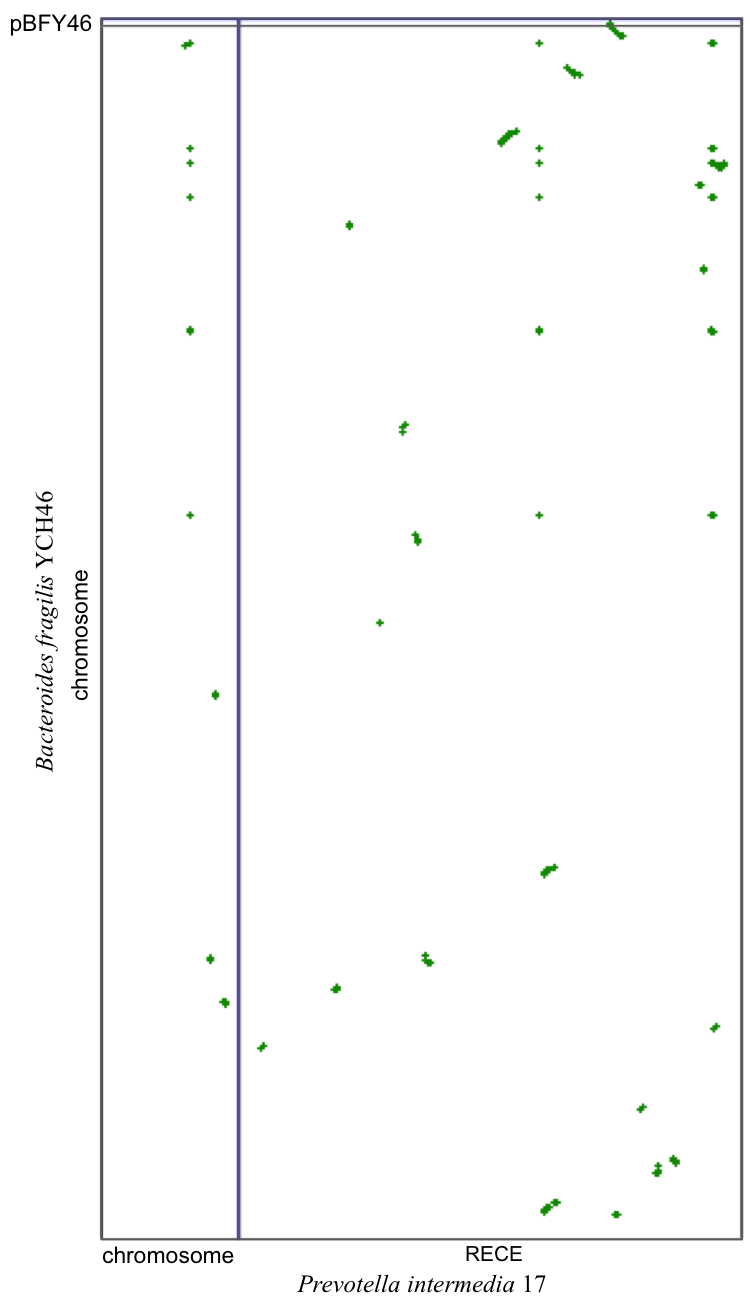
\includegraphics[width=1.1\textwidth]{./img/synteny/new/fig8_15c.png}
   \subcaption{\textit{P. intermedia} 17 (abscisse) \textit{vs.} \textit{B. fragilis} YCH46 (ordonnée).}\label{figsyntprev3}
    \end{minipage}
    \end{center}
    \hspace*{-2cm}
    \begin{minipage}{1.2\textwidth}
    \vspace*{-0.5cm}
   \caption[Synténie de \textit{Prevotella} \textit{vs.} autres Bacteroidetes]{Synténie entre \textit{Prevotella intermedia} 17 et \textit{P. ruminicola} 23 (\ref{figsyntprev1}), \textit{P. denticola} F0289 (\ref{figsyntprev2}), \textit{Bacteroides fragilis} YCH46 (\ref{figsyntprev3}).}\label{figsyntprev}
       \end{minipage}
\end{figure}  

\section{Discussion}
	Cette étude des synténies des génomes multipartites souligne les différences entre RECE et plasmides. \textbf{\color{orange} Les RECE des génomes multipartites possèdent, avec les chromosomes des espèces phylogéniquement proches, des taux de synténie plus importants que les plasmides} (\textit{cf.} résultats pour les plasmides d'\textit{\hyperref[parasti]{Asticcacaulis}, \hyperref[paranab]{Anabaena}, \hyperref[parsphi]{Sphingobium}, \hyperref[parpara]{Dinoroseobacter}} et \textit{\hyperref[paraburk]{Burkholderia}}). Cette constatation est compatible avec soit une formation des RECE à partir de plasmides ``enrichis" en gènes du chromosome par transfert(s) intra-génomique(s), soit une stabilisation sous forme de réplicon d'un fragment de chromosome (\textit{cf.} Chapitre 2, \S \ref{chrIIori}). Cette observation a aussi été retrouvée dans le cas de certains plasmides que nous avons identifiés comme de potentiels RECE (notamment ceux de \hyperref[pararueg]{\textit{Ruegeria} sp. TM1040} et d'\hyperref[parazos]{\textit{Azospirillum brasilense} Sp245}) parmi les plasmides (\textit{cf.} Chapitre \ref{classifsupervisee}), ce qui renforce l'hypothèse d'essentialité de ces réplicons. \\
	Cependant, la structure génomique des RECE diverge plus rapidement que celle des chromosomes \citep{Bavishi2010}. Les taux de synténie entre RECE et chromosomes ont donc été comparés pour des espèces ayant divergé à différents âges (sur la base de leurs relations phylogéniques). Pour de nombreux génomes multipartites, le degré de synténie relatif des RECE par rapport à celui des chromosomes s'atténue lorsque les génomes multipartites sont comparés aux génomes de plus en plus éloignés phylogéniquement. Les génomes multipartites des \hyperref[parvibr]{Vibrionales} et des \hyperref[parburk]{Burkholdériales} en sont des exemples typiques. La structure génomique de ces espèces étant bien documentée (\textit{cf.} Chapitre 2, Table \ref{taborigin}), nos résultats confirment l'origine plasmidique des RECE présents dans ces groupes de bactéries. \\
	L'étude des RECE des \hyperref[parbruce]{Rhizobiales}, lignée également très étudiée, permet de rapprocher les synténies observées entre réplicons à différents événements génétiques: intégration du plasmide ancestral aux RECE, divergences évolutives entre les différents RECE et perte du plasmide ITR originel (ce chapitre, \S \ref{parbruc}). De façon similaire, les résultats obtenus pour les RECE de \textit{\hyperref[parrhod]{Rhodobacter}} et de \textit{\hyperref[parsphi]{Sphingobium}} suggèrent que les deux espèces ont été soumises aux mêmes phénomènes génomiques.\\ 
	Cependant, dans d'autres cas, \textit{\hyperref[parasti]{Asticcacaulis}, \hyperref[paranab]{Anabaena}, \hyperref[parpara]{Paracoccus} et \hyperref[parprev]{Prevotella}}, le signal synténique entre RECE et chromosomes de ces espèces est relativement maintenu et important pour des espèces distantes. Ces RECE semblent de plus posséder une synténie relative (mesurée par l'indice synténique) supérieure à celles des autres RECE étudiés. Pour les RECE d'\textit{Asticcacaulis} et d'\textit{Anabaena}, on constate que la taille relative des régions synténiques des RECE avec les chromosomes d'espèces plus ou moins proches est plus importante que dans le cas de comparaisons entre chromosomes. \textbf{\color{orange} Ces RECE sont donc en contradiction avec les processus génomiques communément utilisés pour caractériser les génomes multipartites:}
\begin{itemize}
	\item Une synténie conservée entre RECE et chromosome contredit l'hypothèse selon laquelle les RECE sont soumis à une évolution plus rapide que les chromosomes, et souligne la conservation et l'importance fonctionnelle de certaines régions de ces RECE. 
	\item Une synténie importante du RECE, voire plus importante relativement que pour le chromosome, avec les chromosomes d'espèces mono- ou multipartites est peu compatible avec l'hypothèse d'``enrichissement" d'un plasmide par transfert(s) intra-génomique(s). Elle est par contre plus cohérente avec celle d'une coupure du chromosome de l'espèce monopartite ancestrale. La structure des régions synténiques des réplicons d'\textit{Asticcacaulis} laisse, de plus, penser que son chromosome et son RECE sont complémentaires, témoignant ainsi d'une scission originelle.
\end{itemize}
	Les taux de variation des régions synténiques entre réplicons sont spécifiques à chaque groupe bactérien. Même si les RECE des Burkholdériales et des Vibrionales découlent vraisemblablement des mêmes processus génomiques, le taux de synténies entre leurs RECE et les chromosomes d'espèces monopartites est plus faible pour les RECE des Vibrionales témoignant de mécanismes génomiques spécifiques à ce groupe bactérien (évolution plus rapide du RECE, transferts intra-génomiques plus rares...).\\
 Les scores de l'indice synténique (éq. \ref{eqsynteny}) peuvent refléter des artefacts génomiques et doivent être interprétés avec prudence. Le score élevé obtenu pour la comparaison du RECE de \textit{Sphingobium} avec le chromosome de \textit{Caulobacter} (Table \ref{tablesyntsphing1}) est fortement influencé par la faible synténie observée entre les deux chromosomes et par la petite taille du RECE comparativement à celle du chromosome, et ne témoigne pas forcément d'une conservation de la synténie chez le RECE.\\
	 Enfin, chez certains groupes d'espèces telles que les cyanobactéries, les signaux de synténie inter-génomes sont trop faibles pour être interprétés. Chez d'autres groupes bactériens, trop peu de génomes sont actuellement disponibles pour permettre une comparaison cohérente. La confirmation des tendances mises en lumière par ces premiers résultats requiert une étude globale approfondie de la synténie inter-génomes avec, pour chaque catégorie de réplicons, un nombre  de génomes.

\iffalse 	  
\fi
